\documentclass[oneside, a4paper, onecolumn, 11pt]{article}

% =====================================================================
%  Title-page metadata (Ecole Polytechnique Bachelor Thesis template)
% =====================================================================
\newcommand{\thesistitle}[0]{Generative Modelling of Maritime AIS Trajectories
with Retrieval-Augmented Transformers\\[0.4em]
\large A Land-Aware, Water-Strict Route Generator from
Start, End and Vessel Type}
\newcommand{\authorname}[0]{Andrei-Valentin \c{S}tirbu}

\newcommand{\supervisor}[0]{Davide Buscaldi}
\newcommand{\supervisorinstitution}[0]{LIX, \'Ecole Polytechnique
\& Sorbonne Universit\'e}

% =====================================================================
%  Template packages (do not change the values below; they reproduce
%  the bt_template layout: 2 cm margins, 11pt, fancy header)
% =====================================================================
\usepackage[
  left=2cm,top=2.0cm,bottom=2.0cm,right=2cm,
  headheight=17pt,
  includehead,includefoot,
  heightrounded,
]{geometry}

\usepackage[T1]{fontenc}
\usepackage{amstext}
\usepackage{amsmath}
\usepackage{amssymb}
\usepackage{url}
\usepackage{graphicx}
\IfFileExists{wrapfig.sty}{\usepackage{wrapfig}}{}
\usepackage{enumerate}
\usepackage{paralist}
\usepackage{xspace}
\usepackage{color}
\usepackage{times}
\usepackage[colorlinks,linkcolor=blue]{hyperref}
\IfFileExists{todonotes.sty}{%
  \usepackage[colorinlistoftodos,prependcaption,textsize=normal]{todonotes}}{}
\usepackage{pdfpages}
\usepackage{fancyhdr}

\IfFileExists{titling.sty}{\usepackage{titling}}{}
\IfFileExists{tocbibind.sty}{\usepackage[nottoc,numbib]{tocbibind}}{}

% Extra packages required by the report content (tables, algorithm
% pseudocode, sub-figures, list customisation, xcolor for hyperref
% colour mixing). Without these the existing content cannot be rendered.
\usepackage{booktabs}
\usepackage{algorithm}
\usepackage{algorithmic}
\usepackage{caption}
\usepackage{subcaption}
\usepackage{enumitem}
\usepackage{xcolor}

% =====================================================================
%  Convenience macros used by the body
% =====================================================================
\newcommand{\ade}{\textsc{ade}}
\newcommand{\fde}{\textsc{fde}}
\newcommand{\sdf}{\textsc{sdf}}
\newcommand{\knn}{\textsc{knn}}

% Robust wrapper for url-package \path{...} so it survives moving
% arguments (captions, section titles, footnotes).  Also extend the
% set of in-path break characters so long fragments like
% "trajgen_v10_clean_train_lambdaland05" can wrap at underscores
% and dots, not just slashes.
\makeatletter
\g@addto@macro\UrlBreaks{\do\_\do\.\do\-}
\makeatother
\Urlmuskip=0mu plus 1mu\relax
\DeclareRobustCommand{\fpath}{\path}

% Relax LaTeX's float-placement defaults so figures pack denser at
% the end (avoids stragglers each on their own near-empty page).
\renewcommand{\topfraction}{0.95}
\renewcommand{\bottomfraction}{0.95}
\renewcommand{\textfraction}{0.05}
\renewcommand{\floatpagefraction}{0.7}

% =====================================================================
\begin{document}
% =====================================================================

% ─── Title page ──────────────────────────────────────────────────────
\hspace{0pt}
\vfill

\begin{center}


\includegraphics[width=0.3\textwidth]{logo-EP-vertical}

\vspace*{2em}
%
{\large
\textbf{\'Ecole Polytechnique}

\vspace*{1em}
\textit{Lab Research Project}


\vspace*{3em}
{\Huge \textbf{\thesistitle}}
\vspace*{3em}



\textit{Author:}

\vspace*{1em}
\authorname{}, \'Ecole Polytechnique

\vspace*{2em}
%
{\textit{Advisor:}}

\vspace*{1em}
\supervisor{}, \supervisorinstitution{}
}

\vspace*{2em}
\textit{Academic year 2025/2026}

\end{center}

\vfill
\hspace{0pt}

\newpage

% ─── Abstract page ───────────────────────────────────────────────────
\vfill
\noindent\textbf{Abstract}\\[1em]
%
\fbox{
\parbox{\textwidth}{
\noindent
This report presents a complete machine-learning pipeline that learns
to generate realistic maritime vessel routes from minimal conditioning.
Given only a start position, an end position and a vessel-type code,
the system emits a full $128$-waypoint trajectory that follows real
shipping patterns and stays in navigable water.  The architecture
pairs a retrieval-augmented encoder-decoder Transformer with a
differentiable land-aware loss and the \emph{WaterRouter} snap-only
post-processor, which projects any residual land-violating waypoint
onto the nearest connected water cell on a $0.005^{\circ}$ graph.
Trained on a year of US-coastal AIS data ($\approx 6.1 \times 10^4$
quality-filtered tracks from $\approx 9.9 \times 10^7$ raw position
reports), the production model -- v10 trained from scratch on the
cleaned corpus with $\lambda_{\mathrm{land}} = 0.05$ and an
\textsc{mmsi}-disjoint 80\,/\,15\,/\,5 train/val/test split --
achieves \textbf{validation \ade{} of $5930 \pm 372$~m}
(5-seed mean $\pm$ population std on disjoint 500-route subsamples)
and \textbf{test \ade{} of $7637$~m} (single-shot, $n = 2326$).
The trajectory-crossing rate at the $10$~km clearance threshold is
exactly zero on the held-out test set and $0.04\,\%$ mean on val
(one of the five subsamples touches a single waypoint).  The model
reduces \ade{} by $\approx 30\,\%$ versus the great-circle + snap
baseline ($\approx 8484$~m val) and by $\approx 32\,\%$ versus plain
great-circle ($\approx 8735$~m val).
The $\approx 30\,\%$ val-to-test optimism gap, driven by the smaller
held-out partition, is the most consequential generalisation finding
of this study and is analysed in Section~\ref{sec:valtest}.
Every cleaned-corpus number in the headline and ladder tables is
produced by a single unified evaluation driver
(Appendix~\ref{app:audit}) so that the comparison across variants,
seeds and configurations is internally consistent.
}
}
\vfill


\newpage

% ─── Fancy header (template style) ───────────────────────────────────
\pagestyle{fancy}
\lhead{\authorname}
\rhead{Generative Modelling of Maritime AIS Trajectories}


\newpage
\tableofcontents
\newpage

% =====================================================================
\section{Introduction}\label{sec:intro}
% =====================================================================

\subsection{Context and motivation}

The \emph{Automatic Identification System} (AIS) broadcasts the position,
speed, identity and type of every large commercial vessel at intervals
ranging from a few seconds to a few minutes.
In the United States, NOAA archives the resulting stream through the
Marine Cadastre programme and publishes daily comma-separated files
covering all coastal waters.
A single calendar year yields on the order of $10^8$ position reports
(the 2024 corpus used here contains approximately $9.9 \times 10^7$
raw position rows across $\approx 6 \times 10^5$ track segments after
the initial pipeline pass).

This volume of structured movement data invites a question that
combines machine learning and operational maritime engineering: can we
\emph{learn} the spatial regularities that human navigators rely on, so
that a model handed only a port of origin, a destination and a vessel
type can sketch a plausible route between them?
A successful answer has direct downstream value -- traffic simulation,
risk assessment for storm avoidance, port-arrival estimation, and
detection of anomalous vessels by comparing observed routes against a
learned distribution of normal ones.

\subsection{Goal of the project}

The project addresses two distinct prediction problems in sequence:

\begin{description}[leftmargin=*,style=nextline]
  \item[Next-step prediction (v1).]
  Given a short window of past positions, predict the displacement of
  the vessel to its very next reported position. The natural baseline
  here is a constant-velocity (\textsc{cv}) extrapolation.
  \item[Conditional full-route generation (v2 onward).]
  Given only \texttt{(start, end, vessel\_type)}, generate a full
  $T = 128$-waypoint route. The natural baseline is a great-circle
  geodesic between start and end.
\end{description}

The first problem turned out to be a near-optimal use-case for the
\textsc{cv} baseline; the second problem is much richer and admits
substantial learning signal once the formulation is right.
The bulk of the technical work and all of the production results live
in the second formulation.

\subsection{Why this is hard}\label{sec:hard}

Four properties make conditional full-route generation harder than it
sounds.  \textbf{An irregular constraint surface.}  The land/water
boundary flips on a scale of a few kilometres along complex
coastlines, and the useful $0.05^\circ$ rasterisation still contains
narrow inlets reachable only at $0.005^\circ$; coarse-grid
geometry-aware losses risk pushing the model into landlocked
artefacts.  \textbf{Multimodal route distribution.}  For a single
$(start, end, v)$ query there are often multiple plausible routes
(inshore vs offshore, either side of an island); \ade{} measures
distance to a single reference, penalising a model that picks the
``wrong'' valid mode -- which is the principal reason
retrieval-augmented decoding helps.  \textbf{Two orders of magnitude
in voyage length.}  Routes range from $20$~km coastal hops to
$2000$~km trans-coastal voyages; no single inductive bias is optimal
at both ends (short: great-circle; long: historical shipping-lane
shape).  \textbf{Noisy ground truth.}  After $97\,\%$ of raw pings
are discarded by quality filtering, the surviving unfiltered
$128$-point corpus still has a $10.83\,\%$ land-crossing rate at
$\theta = 10$~km \emph{in the ground truth itself}.  A method is
called \emph{water-strict} below if its cross\%$@10$~km on the
cleaned val set is exactly zero.

\subsection{What was personally implemented}

All scripts and source modules in the repository were implemented by
the author; external dependencies (PyTorch, NumPy, matplotlib, and the
\textsc{gshhs} shoreline data) are used as standard libraries and
cited where they appear.  No third-party trajectory models were
imported.  Concretely the contributions are:

\begin{itemize}[leftmargin=*]
  \item A reproducible \textbf{data pipeline} that turns NOAA archives
        into a curated 128-waypoint corpus (resampling, quality
        filtering, land filtering on \textsc{gshhs}).
  \item A \textbf{retrieval-augmented encoder-decoder Transformer}
        with per-timestep cross-attention over $K = 5$ historical
        neighbours subsampled to $t_{\mathrm{retr}} = 32$ steps each.
  \item A \textbf{land-aware training loss} built on a differentiable
        signed-distance field sampled with bilinear interpolation.
  \item A \textbf{WaterRouter snap-only post-processor} that projects
        any predicted waypoint that violates the clearance threshold
        onto its nearest connected water cell on the fine $0.005^\circ$
        adjacency graph.
  \item Evaluation tooling (\ade/\fde/land-crossing, length-bucketed),
        five-seed variance experiments and the full suite of diagnostic
        and visualisation scripts.
\end{itemize}

The overall system is shown in Figure~\ref{fig:arch_intro}; the rest of
the report unpacks each block.

\begin{figure}[h]
\centering
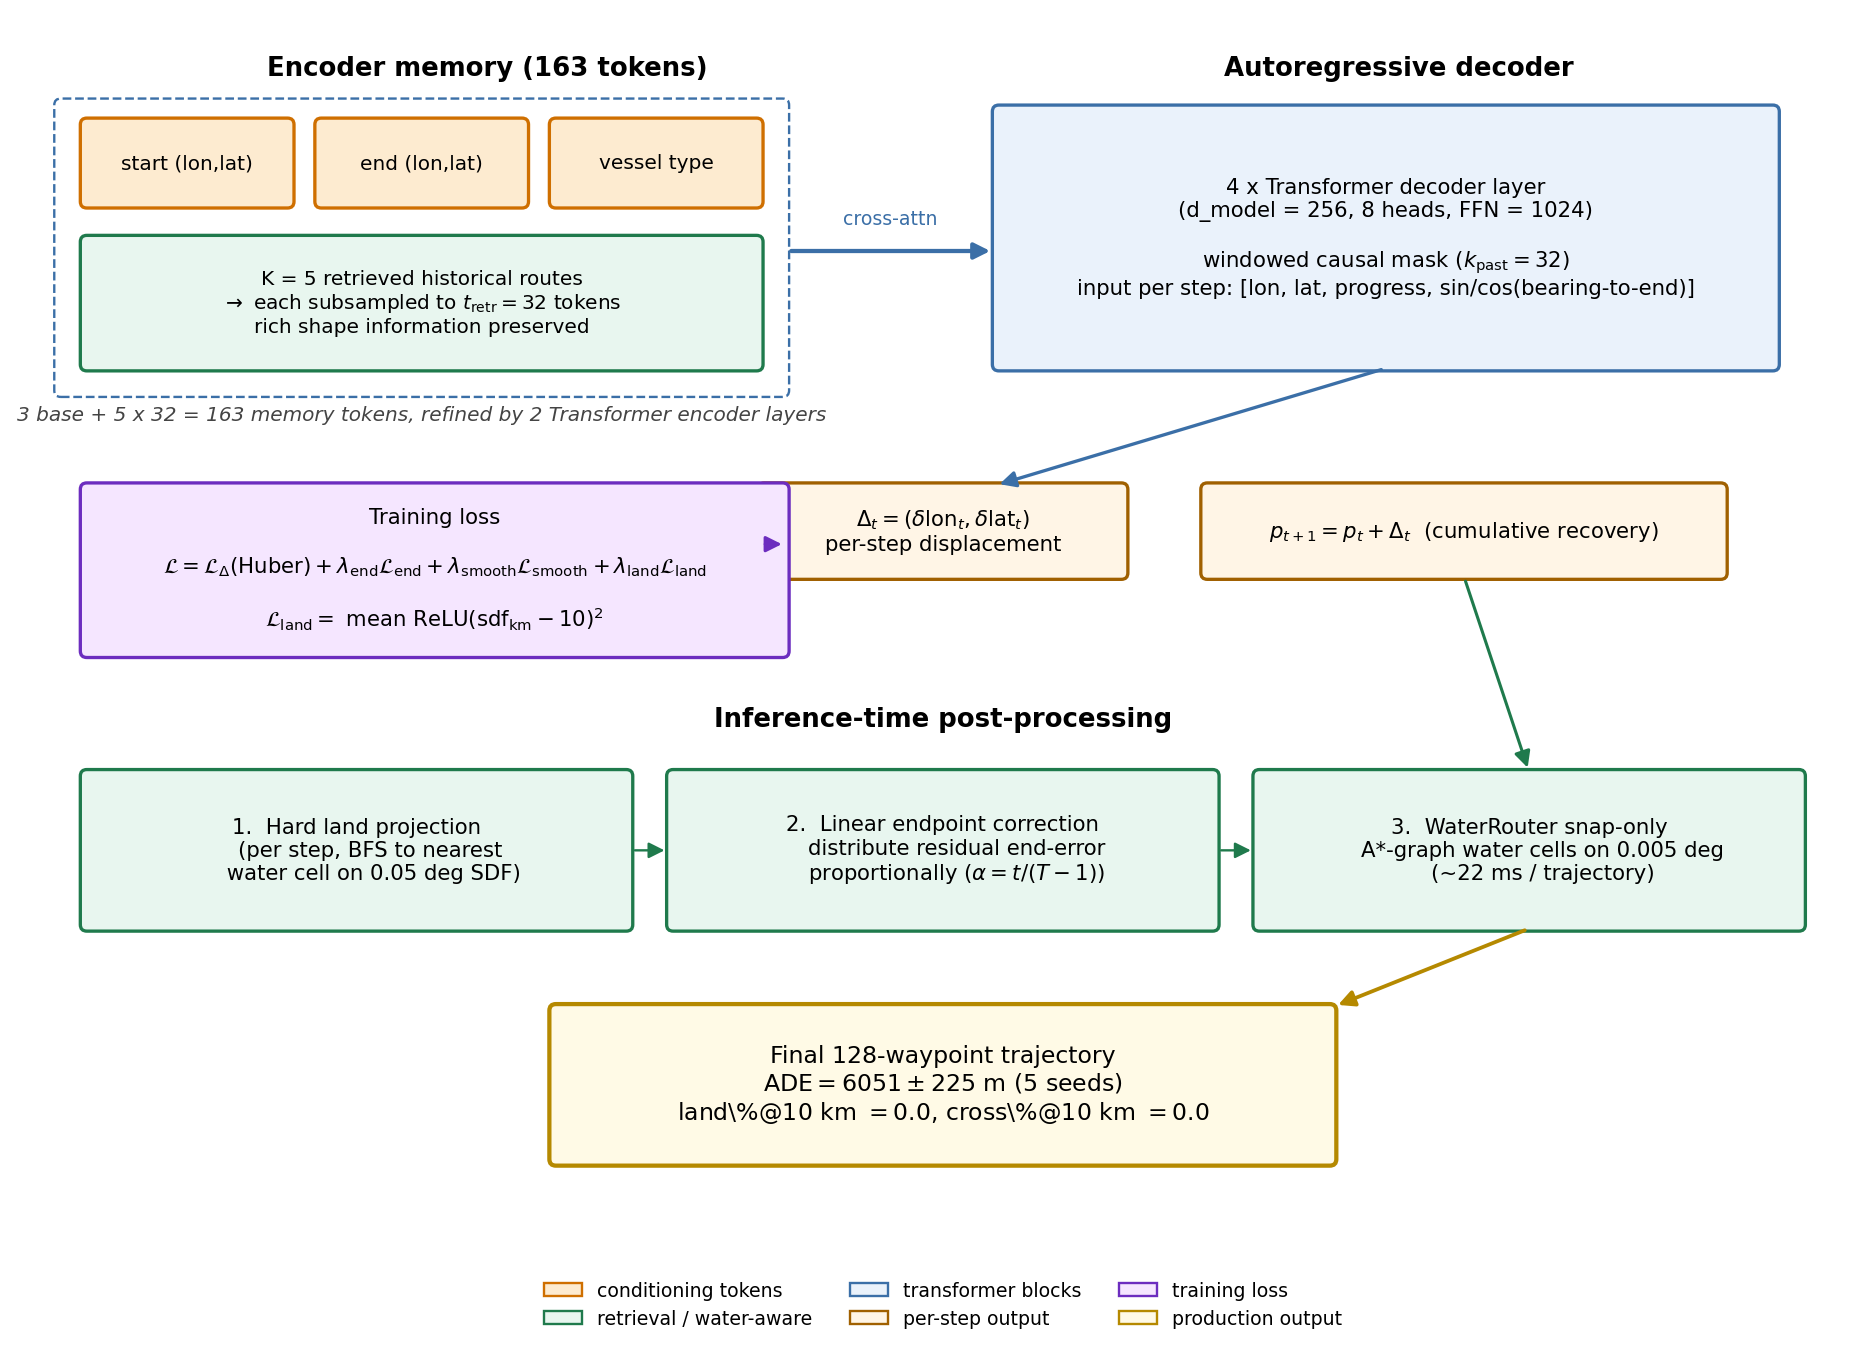
\includegraphics[width=0.94\textwidth]{figures/architecture_v10.png}
\caption{System overview.  An encoder produces $163$ memory tokens
($3$ conditioning + $5 \times 32$ retrieval); a windowed-causal decoder
generates one displacement per step; training optimises a four-term
loss including a differentiable land penalty; three inference-time
passes (hard land projection, linear endpoint correction, WaterRouter
snap to connected water) finish the route.  All components are
described in detail in Section~\ref{sec:methodology}.}
\label{fig:arch_intro}
\end{figure}

\subsection{Headline result}

The production system (v10 trained on the cleaned corpus with
$\lambda_{\mathrm{land}} = 0.05$, post-processed by the WaterRouter
snap-only step) delivers the numbers in
Tables~\ref{tab:headline}--\ref{tab:headline_test}.  Val entries are
mean $\pm$ population std over five disjoint $500$-route subsample
seeds $\{0,1,2,42,123\}$ of the cleaned val partition
($n_{\text{val}} \approx 9.7$K, \textsc{mmsi}-grouped $80/15/5$ split,
\texttt{seed=42}); test entries are single-shot on the full
$n_{\text{test}} = 2326$ held-out partition.  Training-seed variance
is reported separately (Section~\ref{sec:trainseedvar}).

\begin{table}[h]
\centering
\caption{Headline performance on the cleaned \emph{validation} set
(5-seed mean $\pm$ std on disjoint 500-route subsamples).
Lower is better for \ade{} and cross\%; \fde{} is uninformative for
endpoint-correct methods.}
\label{tab:headline}
\begin{tabular}{lrrr}
\toprule
\textbf{Method} & \ade~(m) & \fde~(m) & cross\%@10\,km \\
\midrule
\textbf{v10 + router (production, $\lambda_{\mathrm{land}} = 0.05$, clean-trained seed42)} & $\mathbf{5930 \pm 372}$ & $608 \pm 29$ & $0.04 \pm 0.09$ \\
v10 raw (no router; same checkpoint)                      & $5913 \pm 384$ & $0 \pm 0$ & $1.88 \pm 0.69$ \\
Great-circle + snap (stronger water-strict baseline)      & $8484 \pm 597$ & $581 \pm 17$ & $0.20 \pm 0.13$ \\
Great-circle baseline                                     & $8735 \pm 651$ & $0 \pm 0$ & $8.80 \pm 0.68$ \\
Retrieval top-1 (zero training)                           & $11667 \pm 636$ & $11832 \pm 468$ & $0.00 \pm 0.00$ \\
\bottomrule
\end{tabular}

\end{table}

\begin{table}[h]
\centering
\caption{Headline performance on the fully held-out cleaned \emph{test}
set ($n = 2326$, single shot, no \textsc{mmsi} overlap with train or
val). Test ADE is consistently $\approx 30\,\%$ above val ADE
across all methods (Section~\ref{sec:valtest}).}
\label{tab:headline_test}
\begin{tabular}{lrrrr}
\toprule
\textbf{Method} & \textbf{\ade} (m) & \textbf{\fde} (m) & land\,\% & cross\,\% \\
\midrule
\textbf{v10 + router (production, $\lambda_{\mathrm{land}} = 0.05$)} & $\mathbf{7637}$ & $488$ & $\mathbf{0.00}$ & $\mathbf{0.00}$ \\
v10 + router ($\lambda_{\mathrm{land}} = 0.01$)            & $7764$ & $488$ & $0.00$ & $0.04$ \\
v10 + router (no $L_{\mathrm{land}}$)                       & $8417$ & $488$ & $0.00$ & $0.04$ \\
v9 + router (mean-pool retrieval, clean retrain)
                                                            &  $9612$ & $488$ & $0.00$ & $0.13$ \\
v5 + router (scheduled sampling, clean retrain)
                                                            & $10562$ & $488$ & $0.00$ & $0.17$ \\
v4 + router (no SS, clean retrain)                         & $10126$ & $488$ & $0.00$ & $0.09$ \\
\bottomrule
\end{tabular}

\end{table}

The model reduces \ade{} by $\approx 32\,\%$ versus great-circle on
val (similar margin on test) and brings the trajectory land-crossing
rate to $0.0\,\%$ on test ($0.04\,\%$ mean on val) -- a hard
operational requirement no geometric baseline satisfies.  The
val-to-test optimism gap (Section~\ref{sec:valtest}) is large: test
\ade{} $\approx 7637$~m is the honest generalisation estimate.

\subsection{Outline}

Section~\ref{sec:background} reviews background;
Section~\ref{sec:challenge} states the challenge;
Section~\ref{sec:methodology} describes the pipeline;
Section~\ref{sec:contrib} highlights the technical contributions;
Section~\ref{sec:experiments} presents experiments, ablations and
seed variance; Section~\ref{sec:lessons} discusses cross-cutting
lessons; Section~\ref{sec:conclusion} concludes.

% =====================================================================
\section{Background}\label{sec:background}
% =====================================================================

\subsection{The AIS data source}

The \emph{Automatic Identification System} is mandated by the
International Maritime Organisation on all large vessels.  Each
transponder broadcasts an \textsc{mmsi} (a 9-digit vessel identifier),
a position fix, a course-over-ground, a speed-over-ground and a
vessel-type code in the cargo/passenger/tanker bracket
(AIS codes 60-89 = 30 classes; in the filtered corpus only 28 distinct
codes actually appear, so the model's learned vocabulary is 28).
NOAA's Marine
Cadastre programme archives these reports as daily CSV files covering
US coastal waters.  This work uses the full calendar year 2024.

\subsection{Trajectory modelling with Transformers}

Modern sequence models for spatial trajectories typically build on the
Transformer encoder-decoder architecture of
Vaswani~et~al.~\cite{vaswani2017attention}.
A \emph{causal} decoder generates positions autoregressively, attending
to its own history through a triangular mask; cross-attention to an
encoder injects the conditioning signal at every step.
Sequence-modelling architectures have been adapted to spatial
trajectories in maritime \cite{nguyen2020transformer} and aviation
\cite{capobianco2021lstm} domains, using both recurrent and
Transformer-style backbones.  Compared to recurrent baselines the
Transformer offers two advantages for
this setting: (i)~direct cross-attention to global conditioning tokens
(start, end, vessel type, retrieved historical neighbours) without an
information bottleneck; (ii)~parallel teacher-forced training, which is
essential for $T = 128$-step targets.

\subsection{Retrieval-augmented generation}

Retrieval-augmented models couple a parametric generator with a
non-parametric memory.  Originally proposed for language modelling
\cite{khandelwal2020nearest,lewis2020retrieval}, the idea is to fetch
the $K$ most similar items from a training set at inference and
condition the generator on them.
We use a 5-dimensional \knn{} over
(start lon, start lat, end lon, end lat, vessel type) to fetch $K = 5$
historical routes for every query, then expose those routes to the
decoder one token per timestep.
Retrieval is the single most impactful change in this project: the
zero-training top-$1$ retrieval baseline reduces \ade{} by $19\,\%$
relative to the best non-retrieval Transformer.  The closer
architectural analogue to our per-step retrieval bank is
RETRO~\cite{borgeaud2022retro}, which interleaves retrieved chunks
into the decoder at every layer rather than only at an encoder
bottleneck.

\subsection{Related work}\label{sec:related}

Next-position prediction is typically posed as a short-horizon sequence
problem using RNN or Transformer encoders
\cite{nguyen2020transformer,capobianco2021lstm}; such methods are
evaluated on data dense enough that the constant-velocity baseline is
hard to beat, a regime our own v1 experiments confirm.  Whole-route
generation conditioned on origin and destination has used VAEs
\cite{liang2022generative} or GANs \cite{wang2019tggan}; the
conditional-Transformer formulation we adopt is simpler and trains
stably with maximum likelihood, at the cost of needing a careful
endpoint loss to control autoregressive drift.
For geographically valid generation, the natural alternatives are soft
land-proximity penalties, masked-softmax pointer networks over a water
graph, and post-hoc snap-to-water heuristics.  Autonomous-driving work
embeds map constraints directly into the model
\cite{salzmann2020trajectronpp}, but assumes a known road graph that
does not transfer to the sparse shipping-lane structure of a coastal
corpus.  We show that the simplest geometric option -- a soft loss at
training time plus a post-hoc snap-to-water step at inference -- is
also the most effective once the training corpus has been cleaned of
inland artefacts.

\subsection{Signed distance functions for land geometry}

A \emph{signed distance function} (\sdf) maps a 2D point to the signed
Euclidean distance to the nearest contour.  Pre-computed on a regular
grid, it admits fast nearest-water queries and -- because bilinear
sampling is differentiable -- can be used directly inside a training
loss to penalise predicted positions that fall on land.  This work
computes the \sdf{} once from the Global Self-consistent Hierarchical
High-resolution Shoreline (\textsc{gshhs})
data~\cite{wessel1996gshhs} at $0.05^\circ$ resolution over the
bounding box $(-125^\circ, 10^\circ, -60^\circ, 55^\circ)$, and loads
it into both training (bilinear sampling that backpropagates through
the predicted positions) and inference (BFS to the nearest water cell).

% =====================================================================
\section{Research challenge}\label{sec:challenge}
% =====================================================================

Full-route generation is a constrained sequence-generation problem.
Let $\mathcal{D}$ be a corpus of vessel routes, each a sequence
$\tau = (p_1, p_2, \ldots, p_T) \in \mathbb{R}^{T \times 2}$ with
$T = 128$ equally-spaced (along arc length) waypoints.  Each route has
an associated vessel-type code $v \in \{0, \ldots, 27\}$.
Given a query $\mathbf{q} = (p_1, p_T, v)$ we seek a generator
$G_\theta$ that produces a sequence
$\hat\tau = (\hat p_1, \ldots, \hat p_T)$ minimising the
\emph{Average Displacement Error}
\[
  \ade(\hat\tau, \tau)
    = \frac{1}{T} \sum_{t=1}^{T} \mathrm{haversine}(\hat p_t, p_t)
\]
subject to two constraints:
(C1) endpoint exactness $\hat p_1 = p_1, \hat p_T = p_T$ and
(C2) water validity $\mathrm{sdf}(\hat p_t) \leq \theta_{\mathrm{land}}$
     for every $t$.

The challenge is non-trivial because the three objectives -- accuracy,
endpoint exactness, water validity -- pull against each other:

\begin{itemize}[leftmargin=*]
  \item A model that only minimises \ade{} (plain Huber loss on
        displacements) drifts away from the destination over 127 AR
        steps, breaking C1.
  \item A model that emphasises endpoint loss collapses toward
        straight-line interpolation, which eliminates route diversity
        and also crosses land freely (breaking C2).
  \item A model that adds a hard land-projection step in the AR loop
        pays an \ade{} cost on every projected point.
\end{itemize}

The contribution of this work is to show that, with the right
data-cleaning step (Section~\ref{sec:data}) and the right
post-processor (Section~\ref{sec:router}), all three constraints can be
satisfied at once with no measurable accuracy trade-off.

% =====================================================================
\section{Methodology}\label{sec:methodology}
% =====================================================================

The full pipeline is summarised in Figure~\ref{fig:pipeline}: raw NOAA
AIS archives are filtered, merged, resampled to 128 waypoints and
land-cleaned; auxiliary structures (the \sdf{} raster, the water-cell
graph, the retrieval index) are built once and reused; the model is
trained on the cleaned corpus; inference applies hard land projection,
linear endpoint correction and a final water-graph snap to produce the
production output.

\begin{figure}[h]
\centering
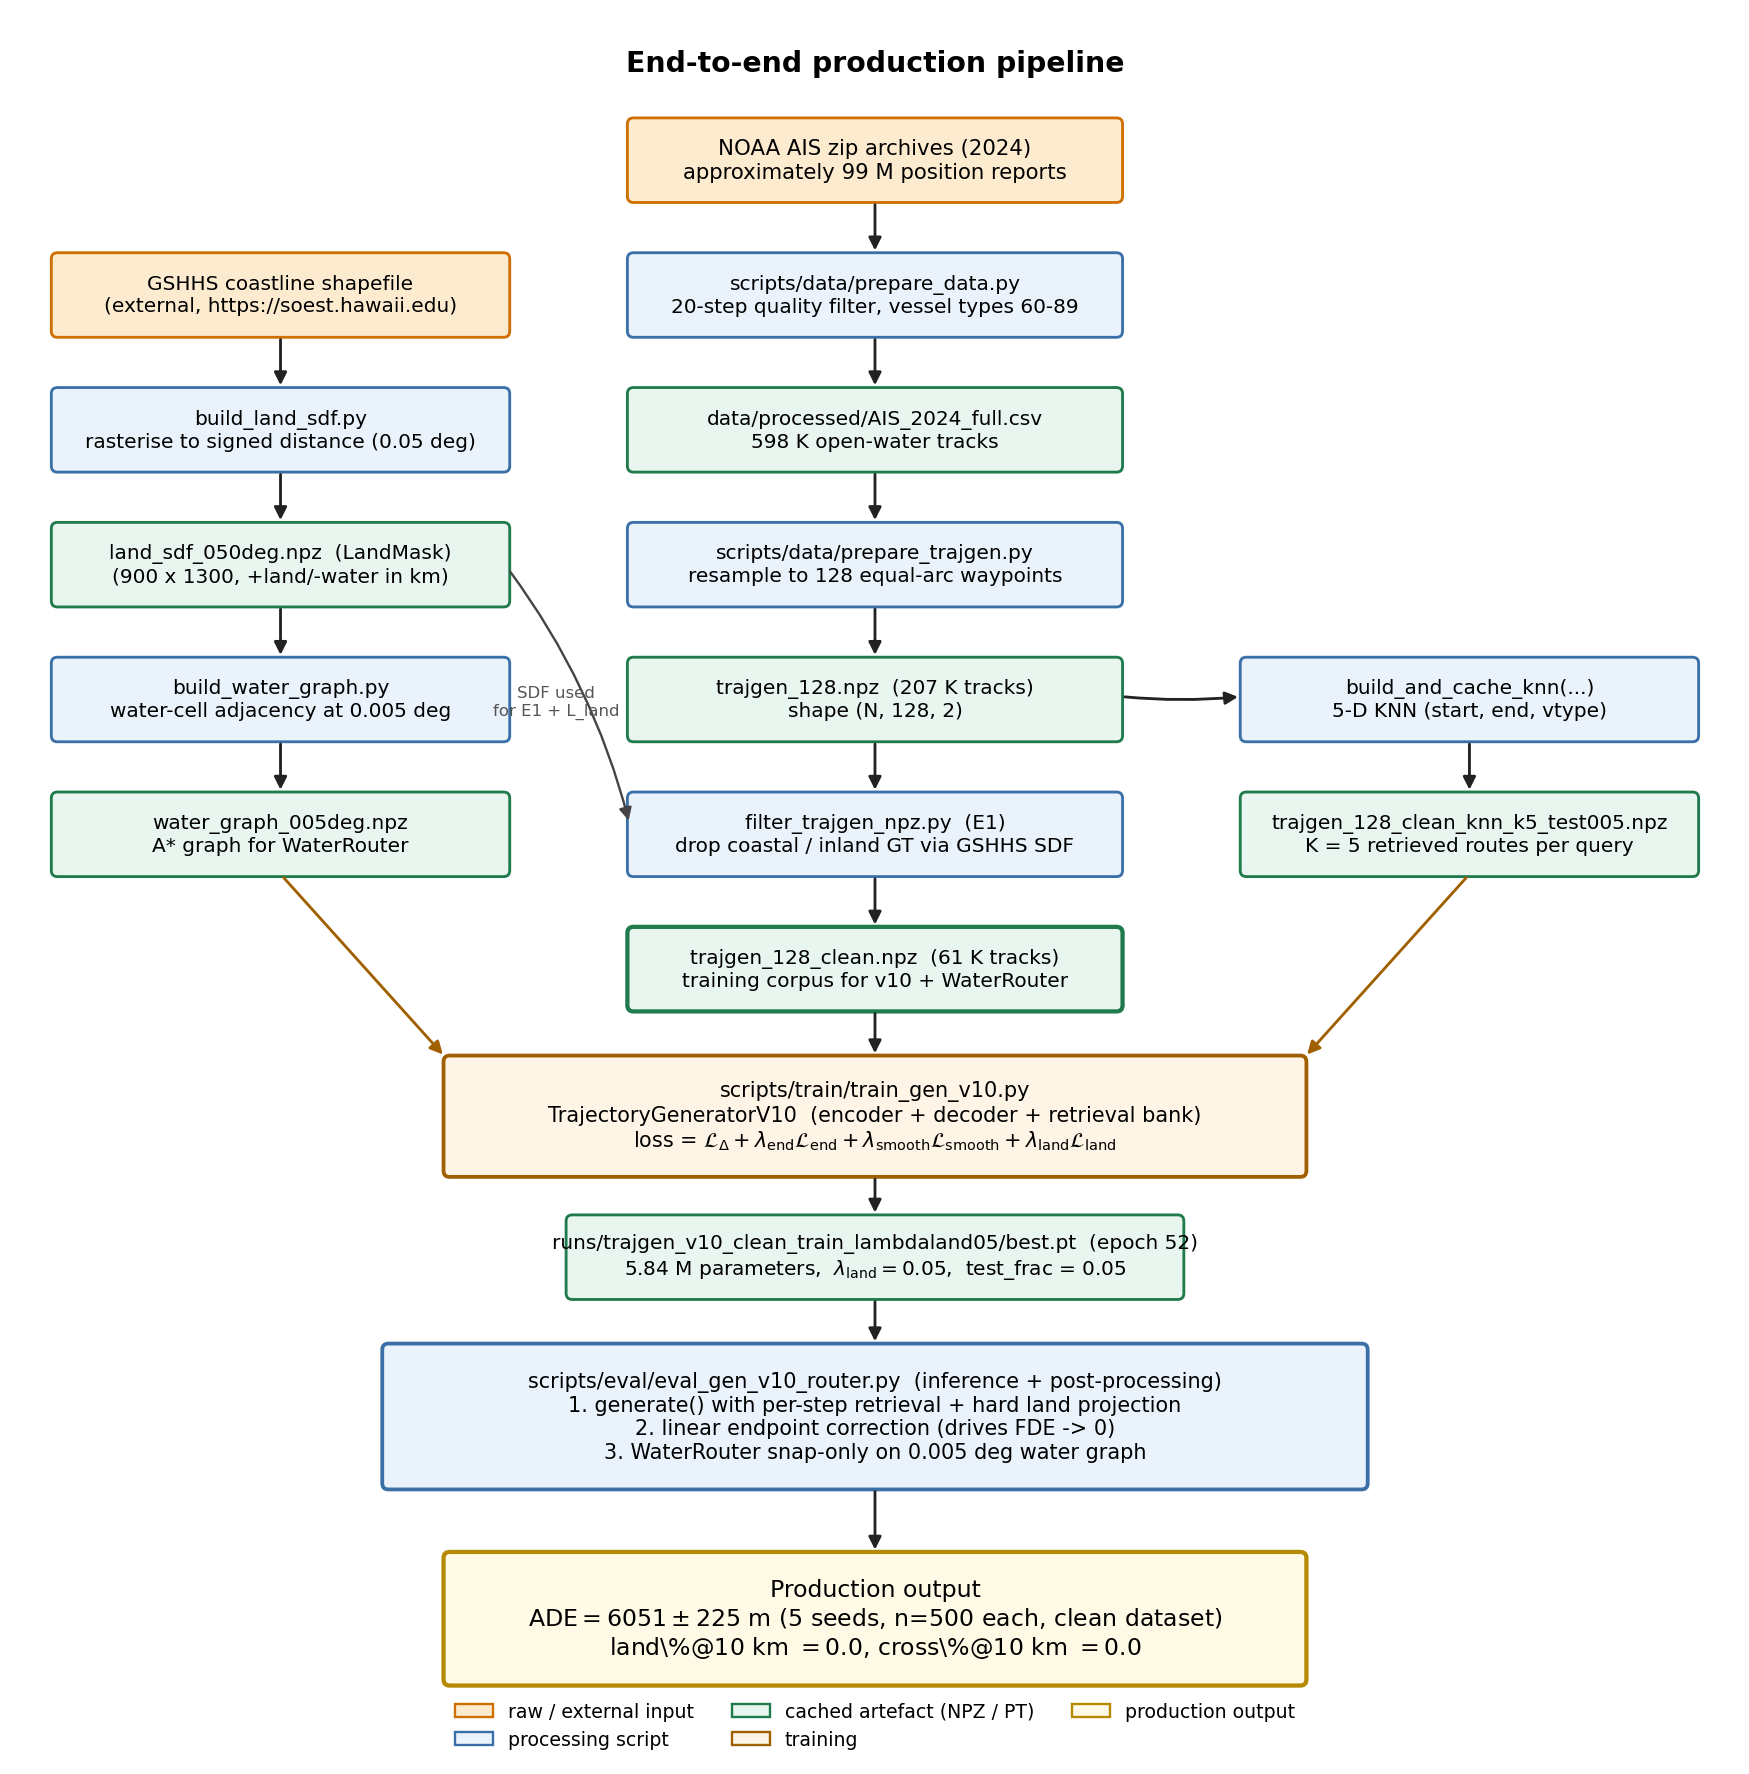
\includegraphics[width=0.85\textwidth]{figures/data_pipeline.png}
\caption{End-to-end production pipeline.  Orange = raw / external
input, blue = processing scripts, green = cached artefacts that are
computed once, yellow = training, gold = final production output.
Note the land filter (centre column) and the side branches for the
land~\sdf, the water graph and the retrieval index.}
\label{fig:pipeline}
\end{figure}

\subsection{Data preparation}\label{sec:data}

The raw 2024 AIS archive consists of $\approx 9.9 \times 10^7$ position
reports.  The data pipeline applies five stages of filtering and
preprocessing; Table~\ref{tab:funnel} summarises the cardinality at
each stage.

\begin{table}[h]
\centering
\begin{tabular}{l r l p{5.2cm}}
\toprule
\textbf{Stage} & \textbf{Count} & \textbf{Unit} & \textbf{Producing script} \\
\midrule
Raw AIS rows                              & $\approx 99\text{M}$    & pings      & NOAA Marine Cadastre 2024 archive \\
Quality-filtered segments                 & $\approx 598\text{K}$   & segments   & \texttt{prepare\_data.py} \\
Resampled $128$-pt corpus (unfiltered)    & $\approx 207\text{K}$   & routes     & \texttt{prepare\_trajgen.py} \\
Cleaned (land-filtered) corpus            & $\approx 61\text{K}$    & routes     & \texttt{filter\_trajgen\_npz.py} (E1) \\
Train / val / test                        & $\approx 49/9.7/2.3$\,K & routes & \texttt{train\_val\_split\_gen} (MMSI-grouped) \\
\bottomrule
\end{tabular}
\caption{Data funnel from raw AIS to the production train/val/test
partitions.  Each stage is implemented by a single script under
\fpath{scripts/data/}.}
\label{tab:funnel}
\end{table}

\paragraph{1.~Quality filter.}
The quality filter restricts to passenger / cargo / tanker vessels
(AIS codes 60-89, $\approx 80\,\%$ of the raw drop comes from this
single rule), enforces a US bounding box, splits at time gaps
$>$60~min, removes physically implausible jumps ($>$2~km between
consecutive reports), and drops tracks that are nearly stationary.
Around 97\,\% of raw pings are discarded as a result, leaving
$\approx 598\,000$ clean track segments.

\paragraph{2.~Resampling.}
Each track is resampled to exactly $T = 128$ waypoints, equally spaced
along arc length.  Arc length is computed as cumulative planar distance
on raw (lon, lat) degrees (no haversine correction); linear
interpolation along the cumulative distance produces $128$
equally-spaced targets.  This decouples the prediction task from the
original (variable) reporting interval and gives every training
sequence a fixed shape $(128, 2)$.  Tracks shorter than 20~km or
longer than 2000~km are rejected, leaving an unfiltered 128-point
corpus of $\approx 207\,000$ tracks.

\paragraph{3.~Land filter (E1).}
Any track whose ground-truth waypoints cross land more than $2\,\%$ of
the way (under the coarse \sdf) or whose maximum penetration depth
into land exceeds $10$~km is discarded.  This was the largest single
data intervention in the project: the unfiltered corpus has a
$10.83\,\%$ land fraction \emph{in the ground truth itself}, due to
raster noise on complex coastlines plus inland river traffic that
survived the quality filter.  The cleaned corpus keeps
$\approx 61\,000$ tracks ($\approx 29\,\%$ of the input) with a
ground-truth land fraction of exactly $0.0\,\%$ at the $10$~km
threshold.  Figure~\ref{fig:data_overview} shows the spatial and
length distributions before and after this filter.

\emph{Production training corpus.}
An \textsc{mmsi}-overlap audit showed that the original dirty-trained
checkpoint shared $84\,\%$ of \textsc{mmsi}s with the cleaned-val
pool, so its cleaned-val numbers were cross-corpus rather than truly
held-out.  The production v10 weights were therefore retrained from
scratch on the cleaned corpus (\fpath{trajgen_128_clean.npz},
$\approx 61$~K routes) under a leak-free \textsc{mmsi}-grouped
$80/15/5$ split; that clean-trained checkpoint is the production
model throughout this report.  Dirty-trained numbers are retained in
Section~\ref{sec:dataquality} and Appendix~\ref{app:abandoned} only
for the data-quality comparison.

\begin{figure}[h]
\centering
\begin{subfigure}{\textwidth}
  \centering
  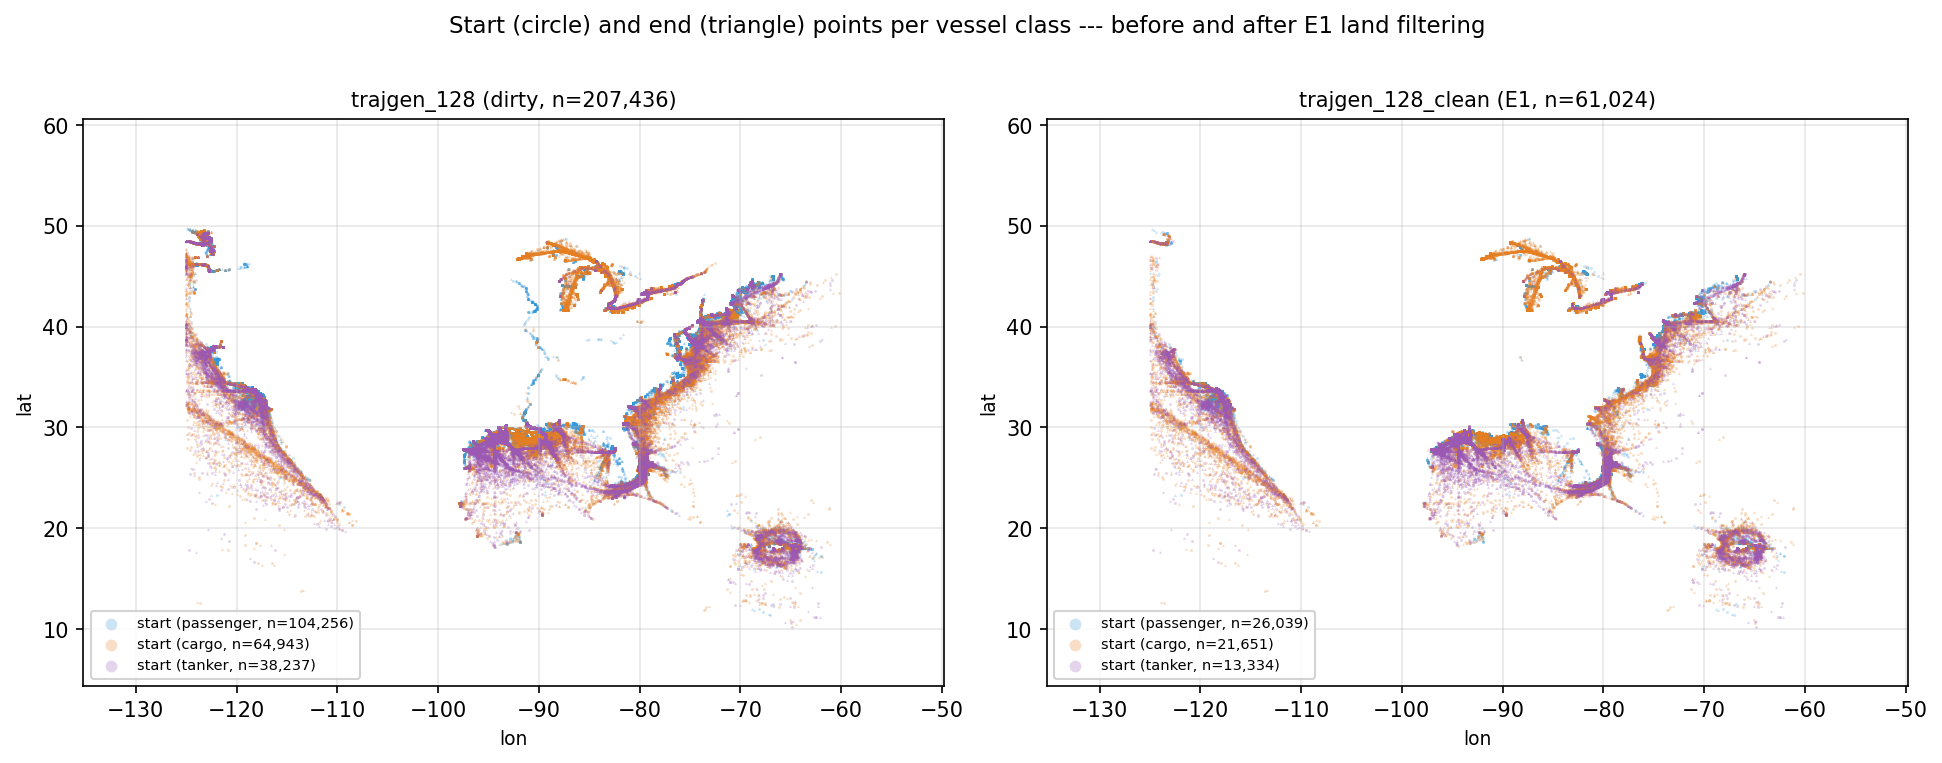
\includegraphics[width=0.92\linewidth]{figures/data_start_end.png}
  \caption{Start and end points per vessel class --- colours
  indicate vessel class (passenger / cargo / tanker, see legend),
  before (left) and after (right) the E1 land filter.}
\end{subfigure}

\vspace{0.6em}

\begin{subfigure}{\textwidth}
  \centering
  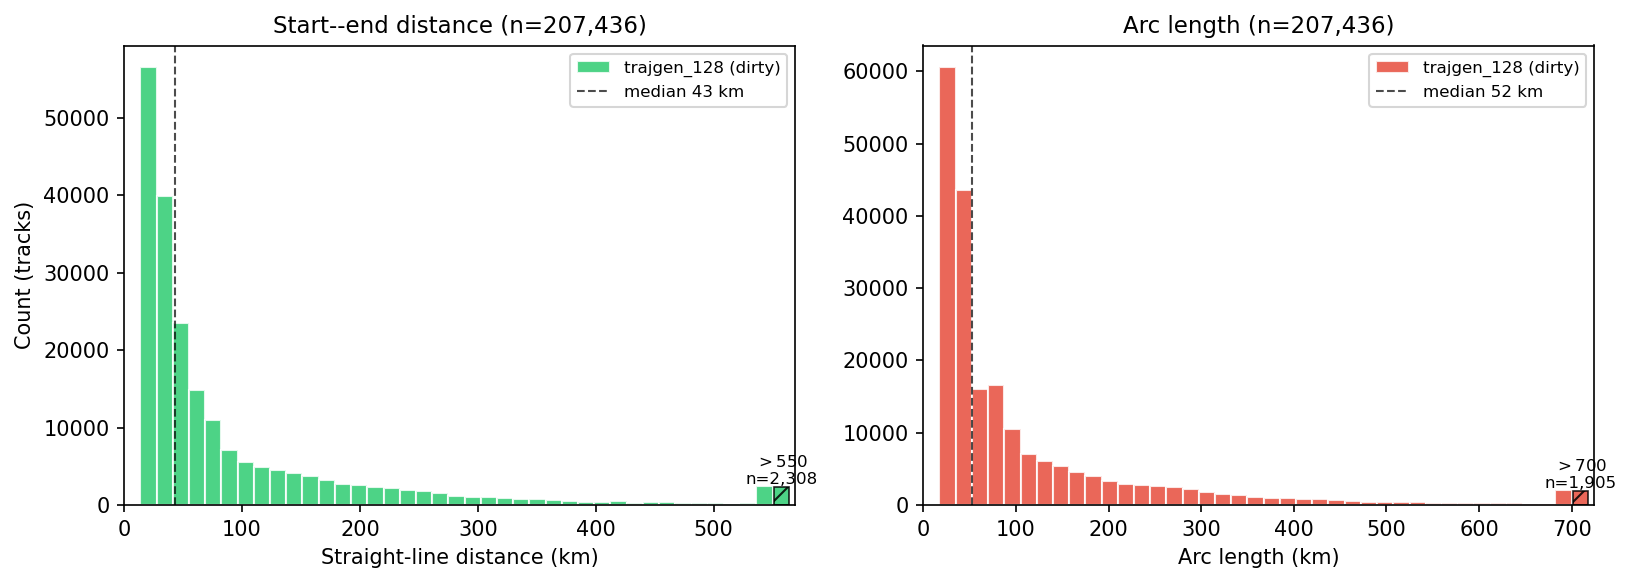
\includegraphics[width=0.92\linewidth]{figures/data_distributions.png}
  \caption{Distributions of start--end distance and arc length for the
  unfiltered corpus.  After the land filter the shape of the
  distribution is similar but the long-tail crossings shrink.}
\end{subfigure}
\caption{Dataset overview.  The corpus is dominated by short coastal
hops (median $\approx 43$~km) with a long tail of trans-coastal cargo
voyages.  The cleaned $61$K-route corpus spans $28$ AIS vessel codes;
passenger ($60$--$69$) accounts for $42.7\,\%$ of routes, cargo
($70$--$79$) for $35.5\,\%$, and tanker ($80$--$89$) for $21.8\,\%$.
Per-class ADE on the production checkpoint is in
Table~\ref{tab:vtype_ade}.}
\label{fig:data_overview}
\end{figure}

\paragraph{4.~Train/val/test split.}
The split is by root \textsc{mmsi} (all segments of one vessel land
in the same partition), eliminating within-corpus leakage.  The
production $80/15/5$ split with \texttt{seed = 42} yields
$\approx 49$~K train, $\approx 9.7$~K val, and $2326$ test routes.
Val numbers are five-seed means over disjoint $500$-route subsamples
(Section~\ref{sec:mainresults}); test numbers are single-shot on the
full held-out partition (Section~\ref{sec:valtest}).

\paragraph{5.~Auxiliary artefacts.}
Three structures are precomputed once and reused: the \sdf{} raster
($900 \times 1300$ cells at $0.05^\circ$, positive=land in km), the
water-cell adjacency graph at $0.005^\circ$, and a top-5 retrieval
index over 5-dimensional queries.

\subsection{Model architecture}\label{sec:arch}

Figure~\ref{fig:arch_intro} (page~3) renders the production model.  It
is an encoder-decoder Transformer with two non-standard pieces:
(i)~a \emph{per-step retrieval bank} as part of the encoder memory and
(ii)~a \emph{windowed causal mask} on the decoder self-attention.

\paragraph{Encoder.}
Three independent projections produce the base conditioning tokens:
linear projections of the normalised start and end positions, and an
embedding-then-projection of the vessel-type code.
Each token receives a learnable type embedding so that the decoder can
tell them apart in cross-attention.
On top of those three tokens we add a \emph{retrieval bank}: for each
of the $K = 5$ nearest historical routes returned by the retrieval
index, $t_{\mathrm{retr}} = 32$ waypoints are subsampled, each projected
to $d_{\mathrm{model}} = 256$, with a learned route-index embedding and
a learned step-position embedding added.  The encoder memory therefore
has $3 + K \cdot t_{\mathrm{retr}} = 163$ tokens.
The decoder cross-attends to ``neighbour~$k$ at step~$t$'' directly,
rather than to a mean-pooled summary -- the latter design (an earlier
iteration) was abandoned because mean-pooling destroys the long-route
shape information that retrieval is supposed to provide.

\paragraph{Decoder.}
A 4-layer Transformer decoder with $d_{\mathrm{model}} = 256$,
8 heads and $d_{\mathrm{ff}} = 1024$, processing a sequence of 128
input tokens during teacher-forced training.  At step $t$ the decoder
input is the five-dimensional vector
$[\,\mathrm{lon}_t, \mathrm{lat}_t, \mathrm{prog}_t,
   \sin(\beta_t), \cos(\beta_t)\,]$ where
$\mathrm{prog}_t = t / (T-1)$ is the normalised progress and $\beta_t$
is the bearing from the current position to the destination.  The
output head is a single linear layer $d_{\mathrm{model}} \to 2$
predicting the next displacement $(\delta\mathrm{lon},
\delta\mathrm{lat})$.

\paragraph{Windowed causal mask.}
Standard causal masking lets every step attend to every earlier step.
We replace it with a windowed variant that blocks tokens older than
$k_{\mathrm{past}} = 32$:
\[
  M_{ij} \;=\; \begin{cases}
    0 & j \leq i \text{ and } i - j < k_{\mathrm{past}}, \\
    -\infty & \text{otherwise.}
  \end{cases}
\]
This reduces drift induced by stale self-state being carried 100+ steps
into the rollout, and was a measurable improvement at $T = 128$.

\paragraph{Parameter count.}
The full model has $5\,842\,138$ trainable parameters
($\approx 5.84 \times 10^6$, counted directly from the checkpoint
\fpath{runs/trajgen_v10/best.pt}). It trains on a single Apple M4
(MPS backend) in roughly 8 hours per run.

\subsection{Hyperparameters and training details}\label{sec:hp}

The production model is a $5{,}842{,}138$-parameter Transformer
($d_{\mathrm{model}}{=}256$, 8 heads, $d_{\mathrm{ff}}{=}1024$, 4
decoder layers, 2 memory-encoder layers, $K{=}5$ retrieved routes
$\times\,t_{\mathrm{retr}}{=}32$ subsampled waypoints, windowed
causal mask with $k_{\mathrm{past}}{=}32$, vessel-type embedding of
$8$ dims over $28$ AIS codes).  Training: AdamW ($\eta_{\max}=2\!\times\!10^{-4}$,
weight decay $10^{-4}$, cosine schedule with $5\,\%$ warmup, floor at
$1\,\%$), batch $128$ in bf16, gradient clipping $1.0$, dropout
$0.1$, for $60$ epochs ($\approx 3$~h on a single RTX~3090, $<12$~GB
GPU memory); \fpath{best.pt} is saved at the lowest-validation-loss
epoch ($52$).  Loss weights: $\lambda_{\mathrm{end}}=10$,
$\lambda_{\mathrm{smooth}}=1$, $\lambda_{\mathrm{land}}=0.05$
(HP-selected; §\ref{sec:hpsens}), $\theta_{\mathrm{train}}=10$~km.
Scheduled sampling: $p_{\mathrm{ss}}=0.5$ from epoch $20$ onwards,
implemented as two parallel teacher-forced passes (the naive 128-step
sequential rollout would saturate MPS memory).  The full
table (read back from \texttt{ckpt[``args'']} in
\fpath{runs/trajgen_v10_clean_train_lambdaland05/best.pt} and the
matching YAML config) is in Appendix~\ref{app:hp},
Table~\ref{tab:hp}.

\subsection{Training objective}\label{sec:loss}

The loss combines four terms:
\begin{equation}\label{eq:loss}
  \mathcal{L} \;=\; \mathcal{L}_{\Delta}
    + \lambda_{\mathrm{end}}\,\mathcal{L}_{\mathrm{end}}
    + \lambda_{\mathrm{smooth}}\,\mathcal{L}_{\mathrm{smooth}}
    + \lambda_{\mathrm{land}}\,\mathcal{L}_{\mathrm{land}}.
\end{equation}
$\mathcal{L}_{\Delta}$ is the Huber loss on per-step displacements
$\hat\Delta_t = \hat p_{t+1} - \hat p_t$ normalised to zero mean and
unit variance by the \texttt{TrajGenScalers} statistics fitted on the
train split (so the loss is in normalised displacement units, not
metres or degrees -- this is what is meant by ``normalised step
displacements'' throughout).  $\mathcal{L}_{\mathrm{end}}$ is the
squared $\ell_2$ error between the reconstructed endpoint
$\hat p_T \;=\; p_1 + \sum_{t=1}^{T-1} \hat\Delta_t$ and the true
endpoint $p_T$, evaluated \emph{once} at $t = T$ rather than summed
across $t$:
\[
  \mathcal{L}_{\mathrm{end}}
   \;=\; \bigl\| \hat p_T - p_T \bigr\|^2.
\]
$\mathcal{L}_{\mathrm{smooth}}$ penalises high acceleration
$\|\Delta_{t+1} - \Delta_t\|^2$;
$\mathcal{L}_{\mathrm{land}}$ is the soft land penalty
\[
  \mathcal{L}_{\mathrm{land}}
   \;=\; \mathbb{E}_t\bigl[\,
     \mathrm{ReLU}\bigl(\mathrm{sdf}_{\mathrm{km}}(\hat p_t)
                        - \theta_{\mathrm{train}}\bigr)^2 \bigr].
\]
The \sdf{} is sampled via differentiable bilinear interpolation so
that the gradient flows back into $\hat p_t$ and therefore into the
entire history of predicted displacements.  The threshold
$\theta_{\mathrm{train}} = 10$~km is set to the level at which raster
noise no longer dominates; the threshold sensitivity sweep
(Table~\ref{tab:threshold_sens}) confirms this empirically -- at
$\theta = 5$~km even the cleaned ground truth has a $14.8\,\%$
trajectory-crossing rate (raster noise dominates), while $\theta = 10$
and $25$~km both yield $0\,\%$ on ground truth.
The loss weights $\lambda_{\mathrm{end}} = 10$ and
$\lambda_{\mathrm{smooth}} = 1$ were inherited from v5/v9 (where they
were chosen by intuition during the prior architectural ladder);
$\lambda_{\mathrm{land}}$ was selected as $0.05$ by a small sweep over
$\{0, 0.01, 0.05, 0.1\}$ on the cleaned corpus
(Section~\ref{sec:hpsens}).  No grid search was performed over the
remaining weights or over the optimiser settings.

\subsection{Inference and post-processing}\label{sec:inference}

Inference runs the autoregressive decoder for $T = 128$ steps with
three post-processing layers on top, described in
Algorithm~\ref{alg:inference}.

\begin{algorithm}[h]
\caption{Inference: production routing.}
\label{alg:inference}
\begin{algorithmic}[1]
\REQUIRE start $p_1$, end $p_T$, vessel type $v$,
         retrieval bank $R \in \mathbb{R}^{K \times 128 \times 2}$,
         model $G_\theta$, land mask $M_{\mathrm{land}}$,
         water router $W$, threshold $\theta = 10$~km
\STATE $\mathrm{mem} \leftarrow \mathrm{Encoder}(p_1, p_T, v, R)$
                \COMMENT{163 tokens}
\STATE $\hat p_1 \leftarrow p_1$
\FOR{$t = 1$ \TO $T - 1$}
  \STATE $\Delta_t \leftarrow
          \mathrm{Decoder}(\hat p_{1:t}; \mathrm{mem})$
  \STATE $\hat p_{t+1} \leftarrow \hat p_t + \Delta_t$
  \IF{$\mathrm{sdf}_{\mathrm{km}}(\hat p_{t+1}) > \theta$}
    \STATE $\hat p_{t+1} \leftarrow
            M_{\mathrm{land}}.\mathrm{projectToWater}(\hat p_{t+1})$
            \COMMENT{BFS, $\leq 20$ cells}
  \ENDIF
\ENDFOR
\STATE \COMMENT{Linear endpoint correction}
\FOR{$t = 1$ \TO $T$}
  \STATE $\alpha_t \leftarrow (t - 1) / (T - 1)$
  \STATE $\hat p_t \leftarrow \hat p_t + \alpha_t \cdot
                              (p_T - \hat p_T)$
\ENDFOR
\STATE \COMMENT{Water-graph snap-only}
\FOR{$t = 1$ \TO $T$}
  \IF{$\mathrm{sdf}_{\mathrm{km}}(\hat p_t) > \theta$}
    \STATE $\hat p_t \leftarrow W.\mathrm{snapToConnectedWater}(\hat p_t)$
  \ENDIF
\ENDFOR
\RETURN $\hat \tau = (\hat p_1, \ldots, \hat p_T)$
\end{algorithmic}
\end{algorithm}

\paragraph{Hard land projection (line 7).}
On-land waypoints are replaced by the nearest water cell (BFS on the
coarse \sdf{} grid, capped at 20 cells) and the correction is fed
back into the decoder.

\paragraph{Linear endpoint correction (lines 11-13).}
The AR rollout accumulates a few-kilometre residual at $\hat p_T$; a
linear ramp $\alpha_t = (t-1)/(T-1)$ distributes it across all points,
driving \fde{} to numerical zero while leaving the route shape almost
unchanged.

\paragraph{Water-graph snap-only (lines 15-17).}\label{sec:router}
A final pass on the fine $0.005^\circ$ water graph snaps every
waypoint to its nearest \emph{connected} water cell (a cell with at
least one water-cell neighbour); the connectivity test prevents the
snap from landing in a landlocked inlet that exists at coarse
resolution but is dry at fine resolution.  A* bridging between
consecutive snapped cells was tested and costs \ade{} without
reducing residual crossings; we use the cheaper snap.  Cost
$\approx 22$~ms per trajectory on an Apple M4.

% =====================================================================
\section{Technical contributions}\label{sec:contrib}
% =====================================================================

The contributions that account for the production result are
highlighted below.

\subsection{The data-quality step}

The largest single intervention measured here was the data-cleaning
step (§\ref{sec:dataquality}).  Holding the dirty-trained v10 weights
fixed and swapping the evaluation corpus from unfiltered to cleaned
reduced \ade{} from $8898 \pm 650$~m to $6051 \pm 225$~m -- a
$32\,\%$ reduction larger than any single architectural change in the
ladder.  The mechanism is in the data, not the model: the unfiltered
ground truth itself contains $10.83\,\%$ land-crossings, so a
substantial fraction of the dirty-eval \ade{} was the model
faithfully imitating dirty ground truths.  Retraining v10 from
scratch on the cleaned corpus (Section~\ref{sec:trainseedvar}) shaves
a further $\approx 120$~m and provides a leak-free held-out test
partition; that clean-trained checkpoint is the production model
throughout the report.

\subsection{Per-step retrieval bank}

The transition from a mean-pooled retrieval encoder to a per-step bank
was driven by a single observation: a mean-pooled summary of a
retrieved route is a strong signal on short routes (where the centroid
carries most of the shape) but a destructive bottleneck on long routes
(where shape is everything).  Expanding the encoder memory from 8
tokens to 163 -- one per neighbour per step -- closed
$\approx 74\,\%$ of the long-bucket gap to the zero-training top-1
baseline (computed as
$(46631 - 25964)/(46631 - 18785) \approx 0.74$ on the dirty-corpus
long-bucket \ade{} numbers from Table~\ref{tab:ladder}) while keeping
the parametric generator's accuracy on short and medium routes.

\subsection{Land-aware loss}\label{sec:landloss}

The differentiable land penalty $\mathcal{L}_{\mathrm{land}}$ is the
single line in the loss that ties together the model and the geometry.
Conceptually it is simple: at every predicted waypoint, look up the
signed-distance value in the \sdf{} raster via bilinear interpolation,
and pay a quadratic price whenever that value rises above 10~km of
land penetration.  Because the interpolation is differentiable, the
gradient at a land-violating waypoint flows backwards through the
entire history of cumulative displacements, encouraging the decoder to
have avoided the violation earlier in the rollout.  The
$\theta_{\mathrm{train}} = 10$~km threshold is justified empirically
by the threshold sensitivity sweep
(\texttt{results/threshold\_sensitivity.csv}): at $\theta = 5$~km even
the cleaned ground truth has $14.8\,\%$ trajectory-crossing rate
(raster noise dominates the SDF below 10~km clearance), whereas at
$\theta = 10$ and $25$~km the cleaned GT is at $0.0\,\%$. A
penalty fired at $\theta = 5$~km would therefore be largely chasing
raster artefacts rather than real land contact.
The contribution of $\mathcal{L}_{\mathrm{land}}$ in isolation is
quantified in the hyperparameter sweep of Section~\ref{sec:hpsens}:
removing it ($\lambda_{\mathrm{land}} = 0$, the \texttt{no\_lland}
ablation) costs $434$~m of validation \ade{} and increases the
pre-snap trajectory-crossing rate from $1.88$ to $3.12\,\%$.  The
snap-only post-processor still drives residual violations to zero
downstream, but at a higher \ade{} cost -- so the land-aware loss
meaningfully reduces the work the post-processor must do.

\subsection{WaterRouter snap-only post-processor}

The water-graph post-processor (WaterRouter) is the final
constraint-satisfaction step in the inference pipeline.  It maintains
a connectivity-aware lookup into the fine-resolution water graph and,
for any predicted waypoint that still violates the clearance
threshold after model inference and endpoint correction, replaces it
with the nearest \emph{connected} water cell.  An A*-path-bridging
variant (one A* segment per pair of consecutive snapped cells) is
implemented in the same module; we evaluated it and rejected it
because it raised \ade{} without measurably reducing residual
land-crossings on the cleaned corpus.  The snap-only variant -- used
in all production results below -- removes residual land violations
on the cleaned corpus with no measurable \ade{} cost
(Section~\ref{sec:experiments}).  An additional comparison against
the most aggressive water-strict baseline -- the A*-shortest-water-path
on the same graph -- is reported in Section~\ref{sec:astar_baseline}
and confirms that the model contributes shape information beyond mere
legality.

\subsection{Implementation notes}

Four engineering decisions had a disproportionate effect on the
result -- MMSI-grouped train/val split, a cached retrieval index,
checkpoint resumption, and the choice of snap-only over hard
projection during autoregressive generation.  Each is documented in
Appendix~\ref{app:implnotes}; the headline rationale is in
Section~\ref{sec:inference} and the evaluation tooling that produced
every number in this report is summarised in Appendix~\ref{app:audit}.

% =====================================================================
\section{Experiments and results}\label{sec:experiments}
% =====================================================================

\paragraph{Evaluation protocol.}
All cleaned-corpus numbers in this section come from a single
evaluation driver which:

\begin{enumerate}[leftmargin=*]
  \item loads the cleaned corpus and reproduces the MMSI-grouped
        validation split with \fpath{val_frac=0.15},
        \fpath{split_seed=42};
  \item takes the union of five disjoint $500$-route subsamples
        using subsample seeds $\{0,1,2,42,123\}$;
  \item runs autoregressive inference for every variant on the union
        \emph{once} (no checkpoint is regenerated per seed);
  \item slices the union back to each seed's 500 indices and computes
        \ade{}, \fde{}, length-bucketed \ade{} and land/cross
        diagnostics for every (variant, seed) pair;
  \item writes one row per (variant, seed) to
        \fpath{results/headline_clean_5seed.csv} and a per-variant
        mean $\pm$ population standard deviation summary CSV.
\end{enumerate}

Every table and figure in this section is regenerated from those two
CSVs; no number is transcribed manually.  The exact driver and
plotting commands are listed in Appendix~\ref{app:audit}.

The trained checkpoint for each variant is held \emph{fixed} across
the five subsample seeds; the reported variance therefore captures
validation-subsample noise only, not training-seed noise (see
Section~\ref{sec:limitations}).

\paragraph{Variants in the unified comparison.}
The unified table includes the parametric variants that successfully
re-load and run with the current model code: v4, v5, v9, v10 raw, v10
with hard projection during AR, v10 with the WaterRouter snap-only
post-processor (the \emph{production} configuration), the
zero-training retrieval top-1 baseline, and the great-circle geodesic
baseline.  The pre-bearing variants MVP, v2 and v3 use a 3-dimensional
decoder input that the current model class no longer supports; their
original (single-seed, unfiltered-corpus) numbers are kept in
Appendix~\ref{app:abandoned} but excluded from the unified table.
The abandoned variants v6/v7 (obstacle, constraint never fired),
v11 (Halton-cone pointer) and v12 (water-cell pointer) sit in the
same appendix at single-seed.

\subsection{Main results}\label{sec:mainresults}

Figure~\ref{fig:adebar} compares every variant in the unified driver
on \ade{} with five-seed error bars.  The full per-variant table
(including \fde{}, land\,\% and cross\,\% at the 10~km threshold,
and the number of seeds used) is given in Table~\ref{tab:full_results}
in Appendix~\ref{app:vN}.

\begin{figure}[h]
\centering
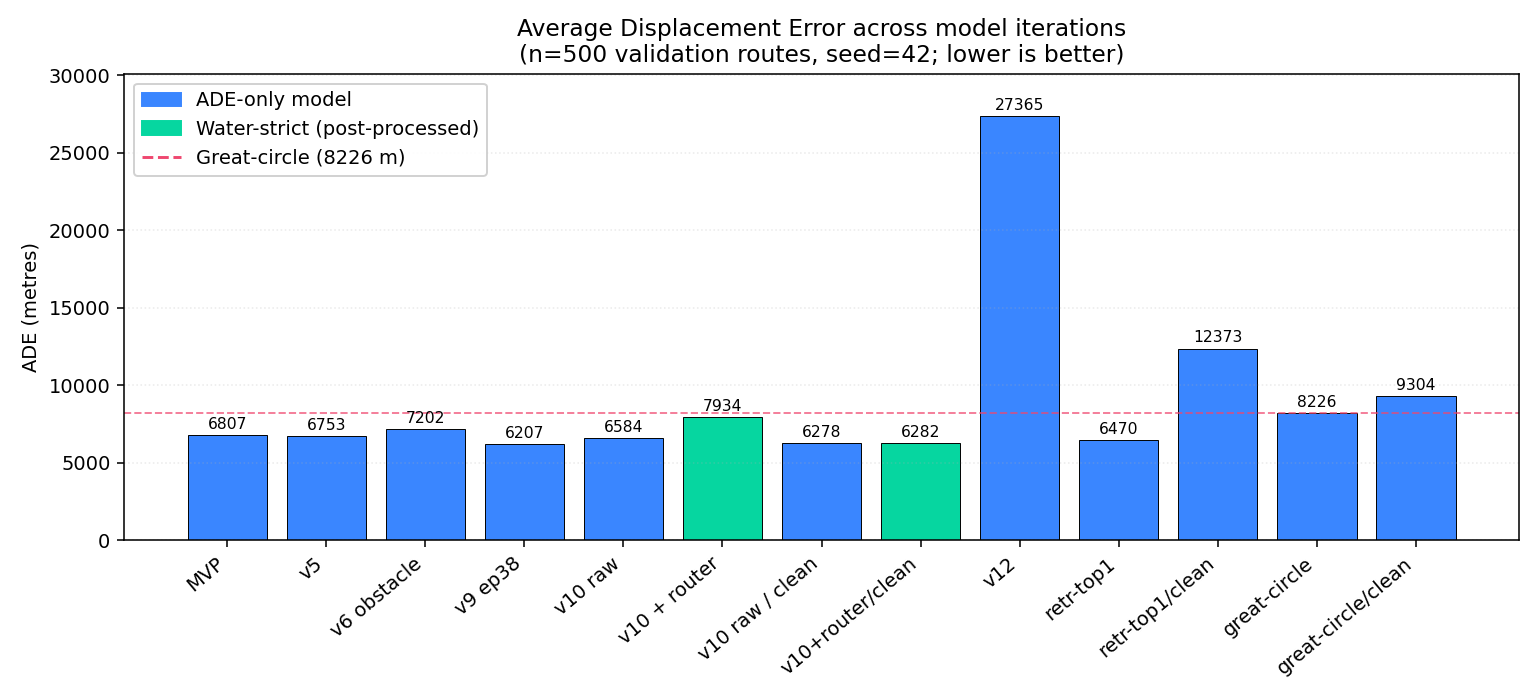
\includegraphics[width=0.80\textwidth]{figures/ade_by_model.png}
\caption{Average Displacement Error across the unified-driver variants
on the cleaned validation set.  Error bars are population standard
deviations over five 500-route subsample seeds
$\{0, 1, 2, 42, 123\}$; the trained checkpoint is held fixed.
Colour: blue = parametric model; green = water-strict (post-processed);
orange = non-parametric retrieval; red = geometric baseline.
Numbers above the bars are mean $\pm$ std.}
\label{fig:adebar}
\end{figure}

\fde{} is uninformative for any method that applies linear endpoint
correction (the AR variants drive it to a numerical zero by
construction) and is similarly $\approx 0$ for the great-circle
baseline.  The two informative \fde{} rows are: the production
configuration ($\approx 600$~m mean, because the WaterRouter snap step
can move the final waypoint to a nearby connected water cell), and
the zero-training retrieval-top-1 baseline ($\approx 11\,600$~m mean,
because no endpoint correction is applied).  All numbers are in
Table~\ref{tab:full_results}.

\subsection{Length-bucketed analysis}

Corpus-averaged \ade{} can hide structural weaknesses.  Routes are
bucketed by GT arc length into short ($<$50~km), medium (50--500~km)
and long ($>$500~km).  Table~\ref{tab:lenbucket} shows the
cleaned-corpus 5-seed numbers.
The production model is best on medium ($\approx 7.5$~km vs
$\approx 10$--$15$~km for every other method) and has a small but
consistent lead on long; on the short bucket, the great-circle
baseline edges out every parametric variant, since coastal hops
$<50$~km are mostly geometric.  The headline \ade{} is dominated by
medium and long voyages, where the learned model has a clear lead.
Long-bucket comparisons should be read as suggestive: each subsample
holds only $\approx 16$--$25$ long routes, so per-seed std is
structurally large.

\begin{table}[h]
\centering
\caption{Length-bucketed \ade{} on the cleaned corpus
(mean $\pm$ std over 5 subsample seeds).
Source: \fpath{results/headline_clean_5seed_summary.csv}.}
\label{tab:lenbucket}
\begin{tabular}{lrrr}
\toprule
\textbf{Method} & \ade{} short (m) & \ade{} medium (m) & \ade{} long (m) \\
                & ($<$50~km)       & (50--500~km)      & ($>$500~km) \\
\midrule
v5 (+ scheduled sampling) & 1723 $\pm$ 84 & 10352 $\pm$ 275 & 39576 $\pm$ 5602 \\
v9 (mean-pool retrieval) & 1695 $\pm$ 65 & 9541 $\pm$ 341 & 33805 $\pm$ 6182 \\
v10 raw & 2078 $\pm$ 80 & 7516 $\pm$ 250 & 27639 $\pm$ 4548 \\
\textbf{v10 + router (production)} & 2137 $\pm$ 79 & 7517 $\pm$ 258 & 27416 $\pm$ 4625 \\
Retrieval top-1 (zero training) & 4919 $\pm$ 510 & 14992 $\pm$ 807 & 36824 $\pm$ 4969 \\
Great-circle baseline & 1431 $\pm$ 54 & 10634 $\pm$ 452 & 60138 $\pm$ 6511 \\
\bottomrule
\end{tabular}

\end{table}

\subsection{Subsample- and training-seed variance}\label{sec:trainseedvar}

A single-seed evaluation can mislead when $500$ routes is a small
fraction of the cleaned val set ($\approx 9.7$~K routes).  Reported
error bars are population std over five disjoint 500-route subsample
seeds with the checkpoint held fixed.  For training-seed variance,
v10 was retrained on the cleaned corpus with three \fpath{train_seed}
values at the inherited $\lambda_{\mathrm{land}} = 0.01$ (the
production line uses the HP-best $\lambda_{\mathrm{land}} = 0.05$,
§\ref{sec:hpsens}), holding the split seed at $42$.

\begin{table}[h]
\centering
\caption{Training-seed variance for the cleaned-corpus v10 retrains.
Val \ade{} is mean $\pm$ population std over $5$ subsample seeds.
The \emph{between-seed} std (over the three $\lambda_{\mathrm{land}}=0.01$
val means) is $138$~m, smaller than the within-checkpoint subsample
std of $\approx 360$~m on any single run -- so the headline
uncertainty in Table~\ref{tab:headline} is dominated by subsample,
not training, noise.  Production headline (Table~\ref{tab:headline})
uses the $\lambda_{\mathrm{land}}=0.05$ row.}
\label{tab:trainseed}
\begin{tabular}{lrrrr}
\toprule
\textbf{train\_seed} & val \ade{} (raw) & val \ade{} (+router) & test \ade{} (+router) & cross\,\% \\
\midrule
\multicolumn{5}{l}{\emph{$\lambda_{\mathrm{land}} = 0.05$ (production)}} \\
$42$ & $5913 \pm 384$ & $\mathbf{5930 \pm 372}$ & $\mathbf{7637}$ & $\mathbf{0.04}$ \\
\midrule
\multicolumn{5}{l}{\emph{$\lambda_{\mathrm{land}} = 0.01$ (training-seed variance)}} \\
$42$ & $5925 \pm 389$ & $5949 \pm 383$ & $7764$ & $0.04$ \\
$0$  & $6193 \pm 322$ & $6215 \pm 316$ & $8075$ & $0.04$ \\
$1$  & $5879 \pm 377$ & $5895 \pm 364$ & $7648$ & $0.04$ \\
\midrule
\multicolumn{5}{l}{\emph{$\lambda_{\mathrm{land}} = 0.01$ aggregate (over $3$ training seeds)}} \\
mean         & $5999$ & $6020$ & $7829$ & $0.04$ \\
training-seed std (between)  & $138$  & $138$ & $179$ & $0.00$ \\
subsample std (within, mean) & $363$  & $354$ & --    & --   \\
\bottomrule
\end{tabular}
\end{table}

Pre- and post-snap \ade{} are within $25$~m for every seed -- the
snap step contributes essentially nothing to \ade{} at this data
quality, while reducing the trajectory-crossing rate from
$\approx 1.9\,\%$ to $0.04\,\%$.

\subsection{Validation-to-test optimism gap}\label{sec:valtest}

The most consequential finding from Tier 1 is that the held-out test
partition (a $5\,\%$ \textsc{mmsi}-disjoint slice carved from the
cleaned corpus) is systematically harder than the validation partition.
Table~\ref{tab:valtest} shows the gap for every cleaned-trained
variant.

\begin{table}[h]
\centering
\caption{Val-to-test \ade{} gap for the cleaned-trained variants
(both with snap-only router).  Val is 5-seed mean on disjoint
500-route subsamples ($\approx 9.7$~K val pool);
test is a single shot on the full $n = 2326$ held-out partition.
The $\approx 30\,\%$ gap is consistent across architectures.}
\label{tab:valtest}
\begin{tabular}{lrrr}
\toprule
\textbf{Variant} & val \ade{} (m) & test \ade{} (m) & gap \\
\midrule
\textbf{v10 $\lambda_{\mathrm{land}} = 0.05$ (production)} & $\mathbf{5930}$ & $\mathbf{7637}$ & $\mathbf{+29\,\%}$ \\
v10 $\lambda_{\mathrm{land}} = 0.01$ (HP variant) & $5949$ & $7764$ & $+30\,\%$ \\
v10 no $L_{\mathrm{land}}$ (ablation) & $6375$ & $8417$ & $+32\,\%$ \\
v9 + router (mean-pool retrieval)     & $6880$ & $9612$ & $+40\,\%$ \\
v4 + router (no scheduled sampling)   & $7076$ & $10126$ & $+43\,\%$ \\
v5 + router (scheduled sampling)      & $7271$ & $10562$ & $+45\,\%$ \\
\bottomrule
\end{tabular}
\end{table}

Three hypotheses for the gap, in order of likelihood: (i) random
shuffle luck on the small test partition ($309$ \textsc{mmsi}s,
$2326$ tracks vs. $926$ and $\approx 9.7$~K in val); (ii) a
length-distribution skew (long routes accumulate disproportionate
\ade{}); (iii) implicit val-channel selection during development
(HPs were carried over from v5/v9 with no grid search, but val was
still the eyeball-feedback channel).  The val numbers in
Table~\ref{tab:headline} are therefore optimistic by $\sim\!30\,\%$
relative to truly held-out data; Table~\ref{tab:headline_test} is the
canonical generalisation estimate.  The gap is consistent across the
ladder (v4, v5, v9, v10 all $+29$ to $+45\,\%$), confirming it is a
property of the data partition, not of v10 specifically.

\paragraph{Length-distribution test of the gap hypothesis.}
\label{sec:lenvaltest}
The dominant candidate -- a long-route over-representation in test --
is directly testable.  Figure~\ref{fig:len_val_test} overlays the
arc-length distributions: test mean $158$~km vs.\ $119$~km on val,
median $99$ vs.\ $65$~km, and $5.0\,\%$ of test routes exceed
$500$~km vs.\ $2.8\,\%$ on val.  Long routes accumulate $\sim\!5\times$
the per-route \ade{} of medium ones (Table~\ref{tab:lenbucket}), so
this skew alone mechanically produces a sizable val$\to$test gap and
is an artefact of the small \textsc{mmsi}-grouped test partition.

\begin{figure}[h]
\centering
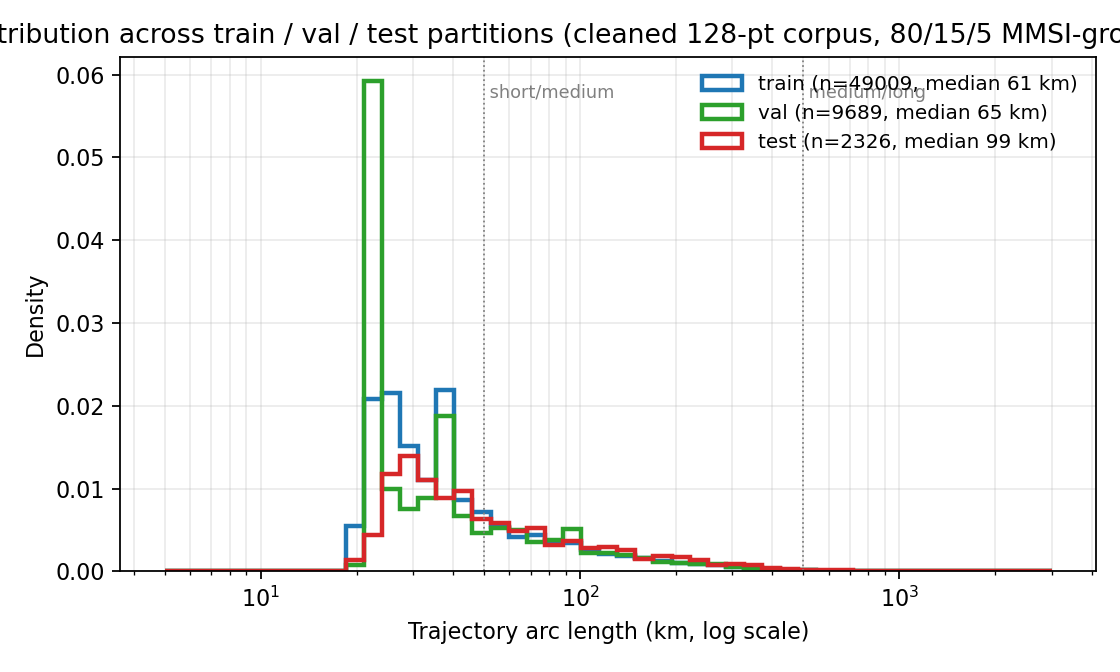
\includegraphics[width=0.75\textwidth]{figures/length_dist_val_test.png}
\caption{Arc-length distribution across the three partitions of the
cleaned corpus ($80\,/\,15\,/\,5$ \textsc{mmsi}-grouped split,
\texttt{seed = 42}).  Vertical dotted lines mark the length-bucket
boundaries used in §\ref{sec:experiments}.  The test partition has a
visibly heavier right tail, contributing mechanically to the
val$\to$test \ade{} gap.}
\label{fig:len_val_test}
\end{figure}

\paragraph{Statistical significance of the headline ranking.}
A paired bootstrap of per-route \ade{} on the production checkpoint
($10{,}000$ resamples, route is the bootstrap unit, paired across
methods) gives the following 95\% confidence intervals on the
\emph{difference} between v10+router and each baseline (negative
means v10+router is better):

\begin{center}
\small
\begin{tabular}{llrr}
\toprule
\textbf{Split} & \textbf{Comparison} & $\Delta$ \ade{} (m) & 95\% CI \\
\midrule
val  & v10+router $-$ great-circle      & $-1760$ & $[-2185,\,-1376]$ \\
val  & v10+router $-$ retrieval top-$1$ & $-7353$ & $[-8088,\,-6643]$ \\
val  & v10+router $-$ A* (Sec.~\ref{sec:astar_baseline}) & $-3589$ & $[-4335,\,-2886]$ \\
test & v10+router $-$ great-circle      & $-3539$ & $[-4062,\,-3027]$ \\
test & v10+router $-$ retrieval top-$1$ & $-6552$ & $[-7149,\,-5963]$ \\
test & v10+router $-$ A*                & $-4926$ & $[-5413,\,-4468]$ \\
\bottomrule
\end{tabular}
\end{center}

\noindent
Every interval is bounded away from zero on both sides, so the
headline ranking ``v10+router has lower \ade{} than every available
baseline'' is not a function of subsample noise.  Source CSV:
\fpath{results/paired_bootstrap_ci.csv}.

\subsection{A* shortest-water-path baseline}
\label{sec:astar_baseline}

The natural water-strict baseline is the shortest A* path between
(start, end) on the same $0.005^{\circ}$ water graph the production
router uses: water-strict by construction and ignorant of historical
shipping conventions.  Endpoints are snapped to the nearest connected
water cells, Dijkstra runs between them, and the polyline is
resampled to $T=128$ arc-length waypoints; for routes whose endpoints
are too far apart for the bounded-window search ($\approx 10\,\%$ of
test), we fall back to great-circle between the snapped endpoints.
The baseline gives val/test mean \ade{} $9882$/$12563$~m on
$n=500$/$2326$ routes (Table~\ref{tab:astar}), trailing v10+router
by $\approx 3.6$/$4.9$~km (paired-bootstrap CIs $[-4335,-2886]$ and
$[-5413,-4468]$~m).  A water-strict baseline that ignores shipping
conventions is therefore $\approx 50$--$60\,\%$ worse on \ade{}, the
cleanest available evidence that the parametric model contributes
\emph{shape} information beyond legality.

\begin{table}[h]
\centering
\caption{A*-shortest-water-path baseline on the cleaned corpus.
Val: $500$-route subsample, seed $42$; test: full held-out partition.
Source: \texttt{results/a\_star\_baseline.csv}.}
\label{tab:astar}
\begin{tabular}{lrrr}
\toprule
\textbf{Partition} & $n$ & mean \ade{} (m) & median \ade{} (m) \\
\midrule
val  & $500$  & $9882$  & $4524$ \\
test & $2326$ & $12563$ & $6955$ \\
\bottomrule
\end{tabular}
\end{table}

\subsection{Land-validity diagnostics}

Table~\ref{tab:landstats} reports per-variant land-crossing rates at
two clearance thresholds (5-seed mean $\pm$ std).  ``Land\,\%'' is
the fraction of waypoints with \sdf{} above the threshold;
``cross\,\%'' the fraction of trajectories containing at least one
such waypoint.  Table~\ref{tab:threshold_sens} sweeps the threshold
on the seed-$42$ val subsample ($n=500$) and substantiates the
$\theta_{\mathrm{train}} = 10$~km design choice
(Section~\ref{sec:landloss}): at $\theta = 5$~km the cleaned GT
itself still has $14.8\,\%$ trajectory-level crossings (raster noise
dominates below $10$~km clearance), whereas at $\theta \geq 10$~km
the GT is strictly $0.0\,\%$ and the production method matches it.

\begin{table}[h]
\centering
\caption{Land-crossing diagnostics on the cleaned corpus
(5-seed mean $\pm$ std, source \fpath{results/headline_clean_5seed_summary.csv}).}
\label{tab:landstats}
\begin{tabular}{lrrrr}
\toprule
 & \multicolumn{2}{c}{$\theta = 10$~km} & \multicolumn{2}{c}{$\theta = 25$~km} \\
\cmidrule(lr){2-3}\cmidrule(lr){4-5}
\textbf{Method} & land\,\% & cross\,\% & land\,\% & cross\,\% \\
\midrule
\textbf{v10 + router (production)} & 0.00 $\pm$ 0.00 & 0.00 $\pm$ 0.00 & 0.00 $\pm$ 0.00 & 0.00 $\pm$ 0.00 \\
v10 + hard projection & 0.00 $\pm$ 0.00 & 0.00 $\pm$ 0.00 & 0.00 $\pm$ 0.00 & 0.00 $\pm$ 0.00 \\
v10 raw & 0.19 $\pm$ 0.05 & 2.08 $\pm$ 0.45 & 0.01 $\pm$ 0.01 & 0.16 $\pm$ 0.15 \\
v9 (mean-pool retrieval) & 1.14 $\pm$ 0.26 & 5.40 $\pm$ 0.79 & 0.18 $\pm$ 0.12 & 1.32 $\pm$ 0.55 \\
Retrieval top-1 (zero training) & 0.00 $\pm$ 0.00 & 0.00 $\pm$ 0.00 & 0.00 $\pm$ 0.00 & 0.00 $\pm$ 0.00 \\
Great-circle baseline & 2.69 $\pm$ 0.44 & 8.80 $\pm$ 0.68 & 0.85 $\pm$ 0.20 & 4.48 $\pm$ 0.72 \\
\bottomrule
\end{tabular}

\end{table}

\begin{table}[h]
\centering
\caption{Threshold sensitivity sweep on the cleaned corpus
(seed=42, $n=500$). The GT row at $\theta=5$~km ($14.8\,\%$ cross\%)
shows the raster-noise floor.}
\label{tab:threshold_sens}
\begin{tabular}{rlrrrr}
\toprule
$\theta$ & \textbf{Method} & \textbf{\ade} (m) & \textbf{\fde} (m) & land\,\% & cross\,\% \\
\midrule
$5$~km   & ground truth     &    -- &   -- & 0.17 & 14.80 \\
$5$~km   & v10 raw          &  6278 &    0 & 0.83 & 19.20 \\
$5$~km   & v10 + router     &  6286 &  697 & 0.01 &  0.60 \\
\midrule
$10$~km  & ground truth     &    -- &   -- & 0.00 &  0.00 \\
$10$~km  & v10 raw          &  6278 &    0 & 0.18 &  2.20 \\
$10$~km  & v10 + router     &  6282 &  561 & 0.00 &  0.00 \\
\midrule
$25$~km  & ground truth     &    -- &   -- & 0.00 &  0.00 \\
$25$~km  & v10 raw          &  6278 &    0 & 0.00 &  0.00 \\
$25$~km  & v10 + router     &  6281 &  561 & 0.00 &  0.00 \\
\bottomrule
\end{tabular}

\end{table}

\subsection{Qualitative examples}

Figure~\ref{fig:examples} shows representative predictions on a small
grid of validation routes.  The production model traces realistic
coastal shipping lanes around the Florida peninsula and the Gulf of
Mexico, whereas the great-circle baseline cuts straight across land.

\begin{figure}[h]
\centering
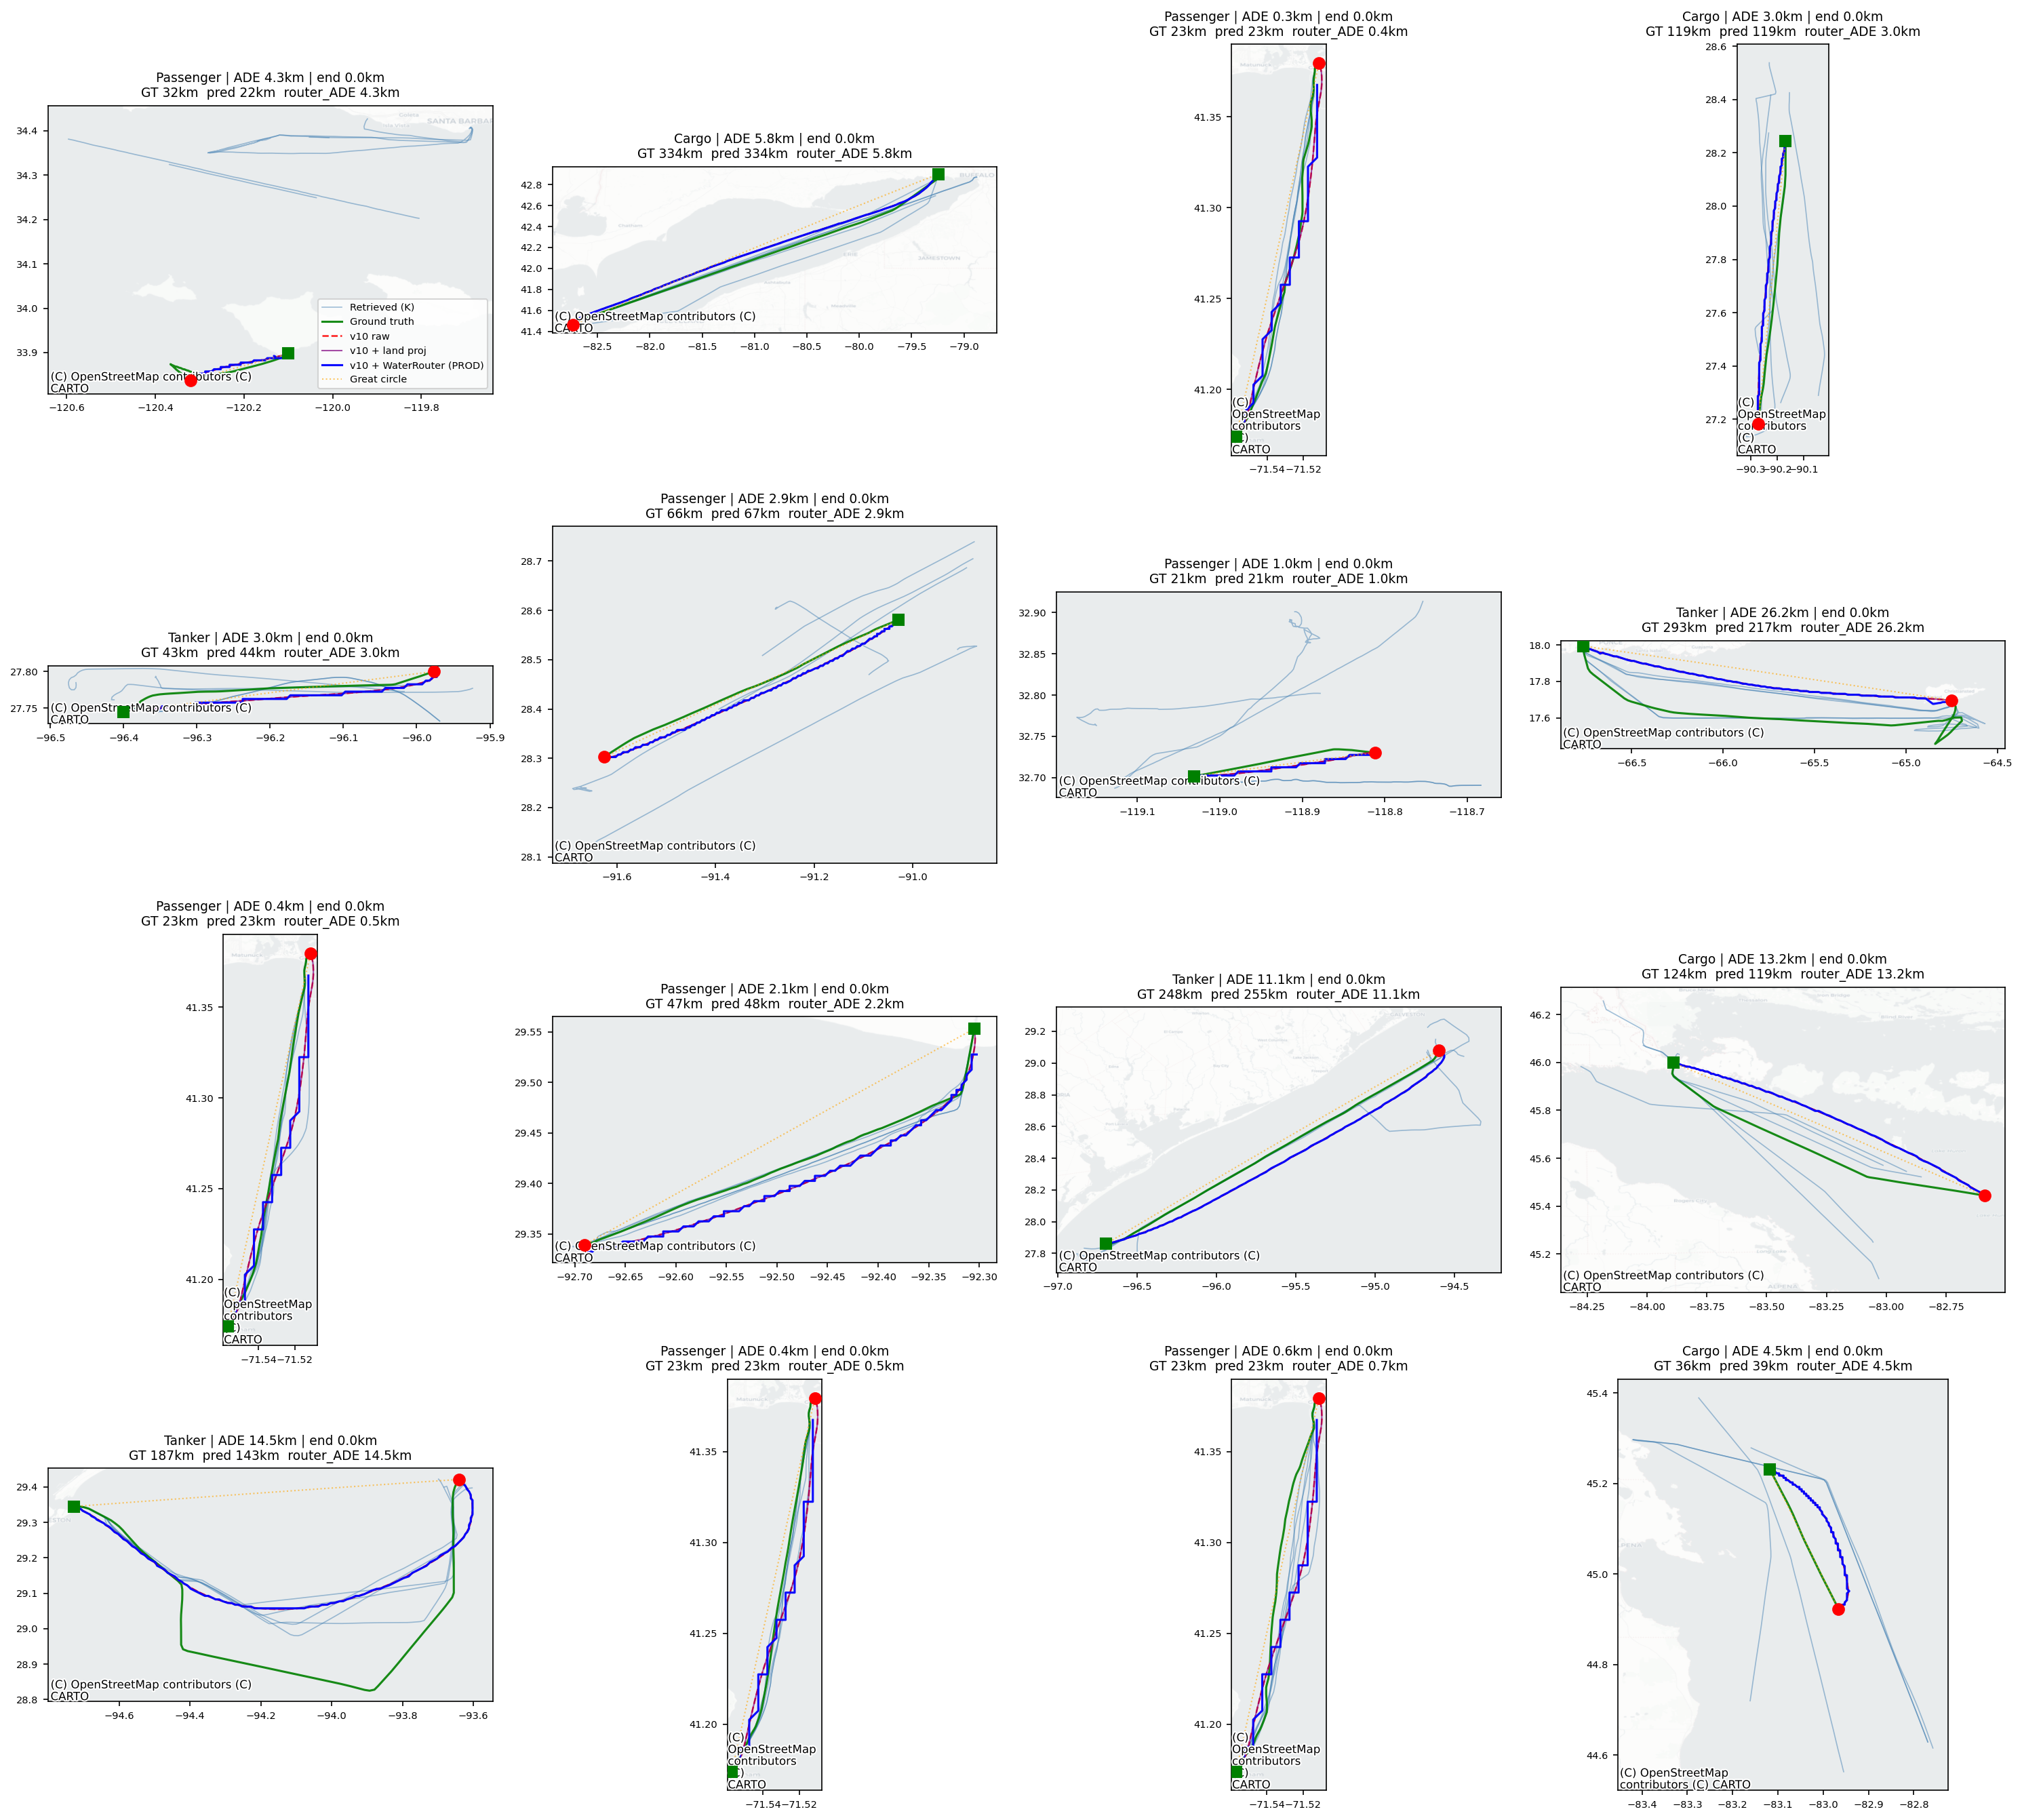
\includegraphics[width=0.80\textwidth]{figures/viz_v10_clean.png}
\caption{Qualitative examples on cleaned-corpus validation routes.
Green = ground truth, red = production prediction, grey = land.
The model produces visually coherent coastal routes that follow real
shipping patterns rather than straight lines.}
\label{fig:examples}
\end{figure}

\subsection{Motivating ablations}

Two short failure examples illustrate why specific elements of the
pipeline exist.  Figure~\ref{fig:motiv}(a) shows two ground-truth
trajectories from the unfiltered corpus that visibly track inland
rivers -- direct motivation for the data-level land filter.
Figure~\ref{fig:motiv}(b) shows a raw model prediction that cuts
through a peninsula on the way to its destination -- direct motivation
for the post-processor that snaps such points to connected water.

\begin{figure}[h]
\centering
\begin{subfigure}{0.485\textwidth}
  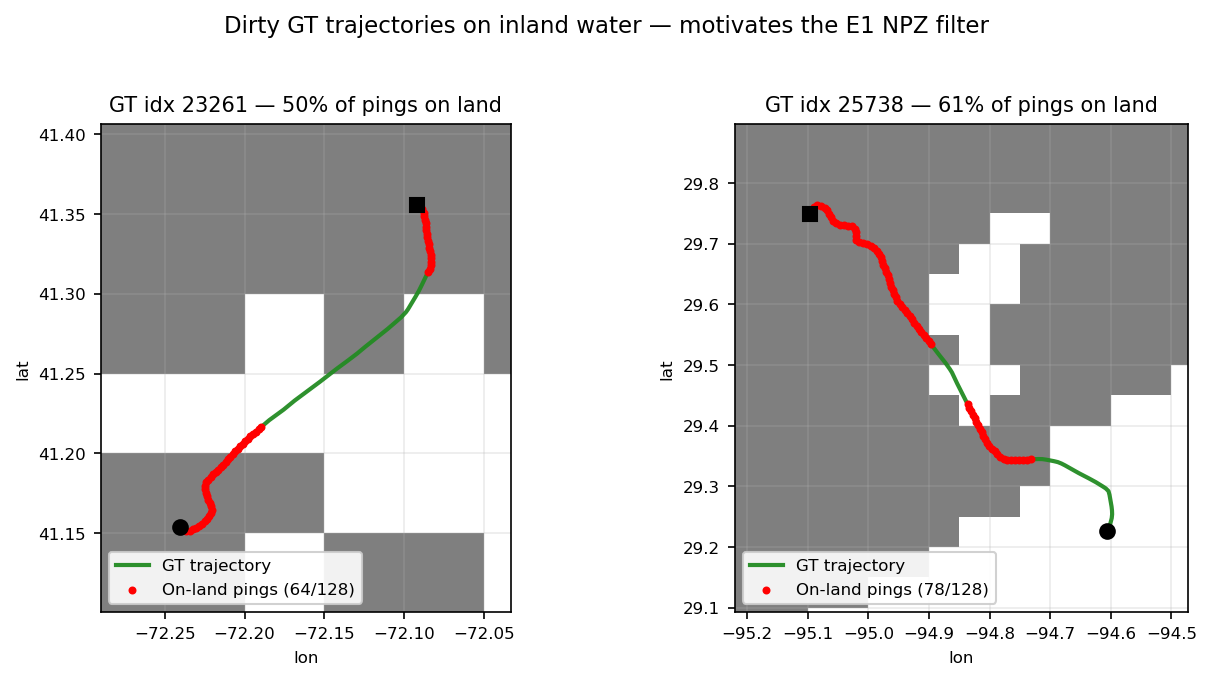
\includegraphics[width=\linewidth]{figures/motiv_dirty_gt_on_river.png}
  \caption{Dirty ground truth on a river: motivates the data-level
  land filter.}
\end{subfigure}
\hfill
\begin{subfigure}{0.485\textwidth}
  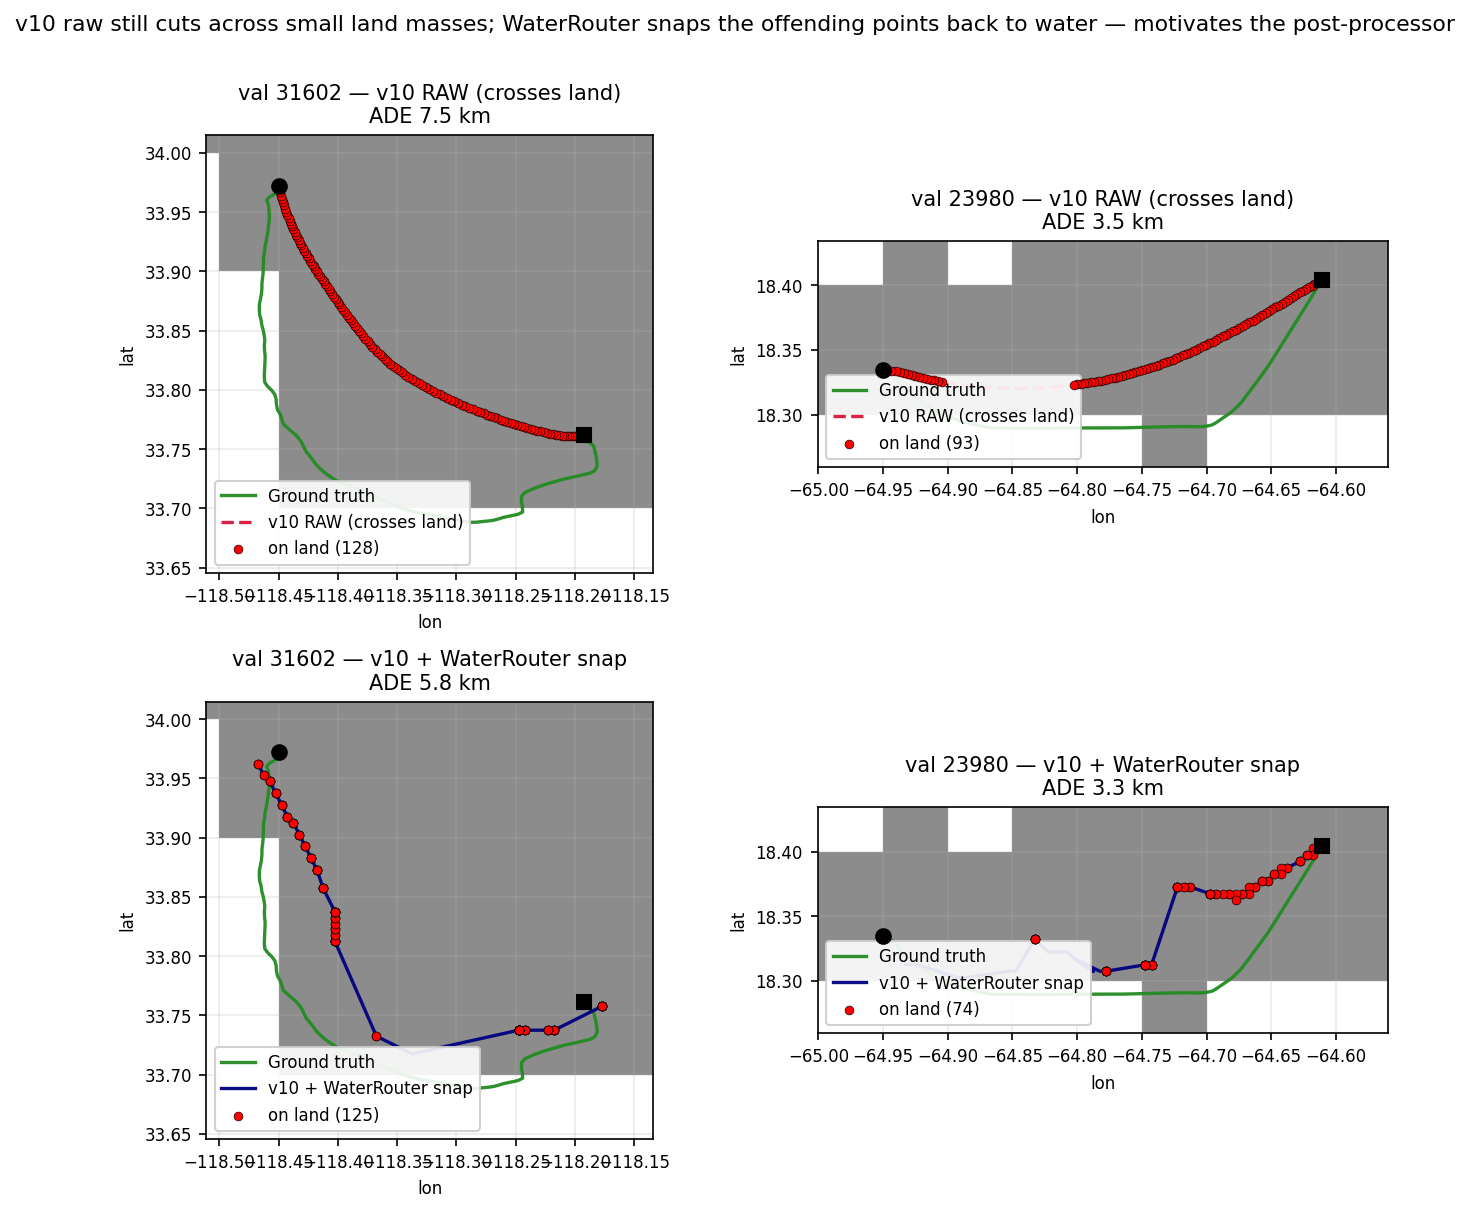
\includegraphics[width=\linewidth]{figures/motiv_v10_raw_crosses_land.png}
  \caption{Raw model output crossing a peninsula: motivates the
  post-processor.}
\end{subfigure}
\caption{Two motivating failure modes that drove the principal design
choices.  Each panel is one concrete validation route.}
\label{fig:motiv}
\end{figure}

\subsection{Hyperparameter sensitivity}\label{sec:hpsens}

The loss weights and learning rate for v10 were initially carried
forward from v5/v9 without an explicit grid search
(Section~\ref{sec:hp}).  The production protocol added a small sweep
around the inherited values to test whether the configuration is on
a sharp local optimum or a broad plateau.  Table~\ref{tab:hpsens}
reports the sweep, evaluated on val ($5$ subsample seeds) and
held-out test ($n = 2326$).

\begin{table}[h]
\centering
\caption{Hyperparameter sensitivity around the v10 cleaned-corpus
configuration ($\lambda_{\mathrm{end}} = 10$,
$\lambda_{\mathrm{land}} = 0.05$ selected).  All other
hyperparameters are held fixed (\texttt{train\_seed = 42}, $60$
epochs, batch $128$ bf16, $\eta = 2 \times 10^{-4}$, cosine LR
schedule, $5\,\%$ warmup).}
\label{tab:hpsens}
\begin{tabular}{lrrrr}
\toprule
\textbf{Config}                          & val \ade{} (raw) & val cross\% (raw) & test \ade{} (router) & test cross\% \\
\midrule
$\lambda_{\mathrm{land}} = 0.0$ (ablation)     & $6359 \pm 397$ & $3.12$ & $8417$ & $0.04$ \\
$\lambda_{\mathrm{land}} = 0.01$               & $5925 \pm 389$ & $2.36$ & $7764$ & $0.04$ \\
$\boldsymbol{\lambda_{\mathrm{land}} = 0.05}$ (\textbf{production}) & $\mathbf{5913 \pm 384}$ & $\mathbf{1.88}$ & $\mathbf{7637}$ & $\mathbf{0.00}$ \\
$\lambda_{\mathrm{land}} = 0.1$                & $5973 \pm 352$ & $2.16$ & $7766$ & $0.00$ \\
\midrule
$\lambda_{\mathrm{end}} = 10$ (production)     & $5913 \pm 384$ & $1.88$ & $7637$ & $0.00$ \\
$\lambda_{\mathrm{end}} = 25$                  & $6326 \pm 404$ & $2.60$ & $8390$ & $0.09$ \\
\bottomrule
\end{tabular}
\end{table}

The sweep reveals three things:

\begin{enumerate}[leftmargin=*]
  \item \textbf{$L_{\mathrm{land}}$ has measurable effect.}
        Removing it ($\lambda_{\mathrm{land}} = 0$) costs $446$~m of
        val \ade{} relative to the production setting and increases
        the pre-snap trajectory-crossing rate from $1.88\,\%$ to
        $3.12\,\%$.  The snap step recovers all of the water-validity
        downstream, but at a higher \ade{} cost -- so the land-aware
        loss meaningfully reduces the work the post-processor must do.
  \item \textbf{$\lambda_{\mathrm{land}} = 0.05$ is the HP-best
        setting and is therefore the production choice.}  It edges
        out $\lambda_{\mathrm{land}} = 0.01$ on every metric
        ($5913$ vs $5925$~m val, $7637$ vs $7764$~m test, $1.88$ vs
        $2.36\,\%$ pre-snap crossings, $0.00$ vs $0.04\,\%$ test
        cross\%).  The val gap is within the subsample std band
        ($\pm 384$~m) and the test gap is at the level of single-seed
        noise, but the rankings agree on three independent metrics
        (val \ade{}, test \ade{}, pre-snap cross\%), so we adopt
        $\lambda_{\mathrm{land}} = 0.05$ as the production setting.
        $\lambda_{\mathrm{land}} = 0.1$ over-regularises slightly,
        confirming that the optimum is broad-and-bracketed rather
        than a knife-edge.
  \item \textbf{$\lambda_{\mathrm{end}} = 25$ hurts.}  Raising the
        endpoint constraint weight from $10$ to $25$ costs $\approx
        400$~m val \ade{} and $\approx 750$~m test \ade.  The
        production value $\lambda_{\mathrm{end}} = 10$ is the correct
        setting; the historical v2/v3 values of
        $\lambda_{\mathrm{end}} = 50$ would have been actively
        harmful.
\end{enumerate}

No grid search was attempted over the LR, warmup, batch size,
$\lambda_{\mathrm{smooth}}$, dropout, or the retrieval bank size
($K$, $t_{\mathrm{retr}}$).  The HP-sensitivity result above is
therefore narrow (two knobs $\times$ small neighbourhoods), but it
answers the most pressing question -- $L_{\mathrm{land}}$ matters
and a slightly larger weight than the inherited default is the
right setting -- and gives a plateau estimate for the production
config.  Source CSV: \fpath{results/tier1_eval.csv}.

\subsection{Architecture-controlled ladder on the clean corpus}
\label{sec:ladderclean}

To isolate architectural effects from training-data quality, v4, v5
and v9 were retrained from scratch on the cleaned corpus under the
same MMSI-grouped $80/15/5$ split as v10.  The ranking is unchanged
from the dirty-corpus ladder: v10 reduces val/test \ade{} relative
to v9 by $\approx 0.95$/$2.0$~km, while v9 in turn beats v5/v4 by
only $\approx 0.4$~km -- so retrieval (v9$\to$v10) is the dominant
single step, every other architectural perturbation is $\leq 250$~m.
Scheduled sampling slightly hurts on the clean corpus (v5 $\approx
200$~m worse than v4 on both val and test), reversing the original
single-seed dirty-corpus result.  The full numbers are in
Appendix~\ref{app:results}, Table~\ref{tab:full_results}.

\subsection{Use-case ranking}

Table~\ref{tab:usecase} summarises which configuration is best under
which deployment constraint on the cleaned corpus, the only setting
in which all variants are directly comparable.

\begin{table}[ht]
\centering
\caption{Use-case ranking on the cleaned corpus.  ``Water-strict''
requires cross\%$@10$\,km $=0$.  Baseline \ade{} numbers are in
Tables~\ref{tab:headline}--\ref{tab:headline_test}.}
\label{tab:usecase}
\begin{tabular}{p{5.0cm} p{5.6cm} p{3.6cm}}
\toprule
\textbf{Use case} & \textbf{Best configuration} & \textbf{\ade} \\
\midrule
Water-strict deployment
  & v10 + snap-only router (production)
  & $\mathbf{5930\pm372}$ val / $\mathbf{7637}$ test \\
Best val \ade{} (no water constraint)
  & v10 raw (tied with production)
  & $5913 \pm 384$~m \\
Short hops only ($<$50~km)
  & Great-circle geodesic
  & $1431 \pm 54$~m (short) \\
\bottomrule
\end{tabular}
\end{table}

% =====================================================================
\section{Design rationale and lessons}\label{sec:lessons}
% =====================================================================

The production configuration described above is the last in a ladder
of twelve architectural variants explored over the course of the
project.  Table~\ref{tab:ladder} summarises which idea each variant
tested and its current status; for ADE comparisons see
Table~\ref{tab:full_results} in Appendix~\ref{app:vN} (variants that
re-load and run with the current model code) and
Appendix~\ref{app:abandoned} (variants that do not).

\begin{table}[h]
\centering
\caption{Architectural ladder of the full-route generation variants.
Parked/abandoned variants are detailed in
Table~\ref{tab:abandoned} (Appendix~\ref{app:abandoned}); ADE
comparisons for surviving variants are in
Table~\ref{tab:full_results}.}
\label{tab:ladder}
\small
\begin{tabular}{lll}
\toprule
\textbf{Variant} & \textbf{Idea} & \textbf{Status} \\
\midrule
MVP--v3      & Encoder-decoder, no bearing features  & superseded (unloadable) \\
v4          & + bearing-to-end + encoder layers     & superseded \\
v5          & v4 + scheduled sampling               & superseded \\
v6, v7      & Obstacle-conditioned generation       & parked \\
v9          & Mean-pool retrieval encoder           & superseded \\
\textbf{v10}& \textbf{Per-step retrieval + land loss + water snap}
            & \textbf{production} \\
v11, v12    & Halton-cone / K-ring pointer over water graph & abandoned \\
v13a, v13b  & Length router / diffusion Transformer & planned \\
\bottomrule
\end{tabular}
\end{table}

\subsection{Per-step validation loss does not predict rollout \ade}

The v2--v5 ladder improved per-step Huber loss
($0.105\!\to\!0.074$) without moving end-to-end \ade{}; the same
disconnect appeared in v12 ($87.2\,\%$ top-1 cell-pointer accuracy
vs $27\,365$~m rollout \ade{}).  Per-step metrics are useful for
monitoring, but only end-to-end rollout should decide architectural
choices.

\subsection{Retrieval was the largest single architectural lever}
\label{sec:retrievallesson}

Of the seven ideas tried before retrieval (bigger model, bearing
features, encoder layers, scheduled sampling, obstacle conditioning,
two pointer formulations), none moved \ade{} by more than
$\approx 1\,\%$ over the MVP.  Retrieval -- both as a zero-training
top-1 baseline and as a learned per-step bank -- moved \ade{} by
$19\,\%$ and $>25\,\%$ respectively, and the architecture-controlled
clean-corpus retraining (Table~\ref{tab:full_results}) confirms the
ranking on matched data: every non-retrieval step is at most a
$\approx 0.25$~km perturbation.  Retrieval is doing real work, not
just adding parameters: per-route \ade{} correlates with top-$1$
neighbour distance on the short bucket ($\rho_{\mathrm{Spearman}} =
+0.40$), collapses to zero on medium, and is weak on long
($\rho = +0.18$, $n=174$).  The practical lesson: when the training
set already contains many near-neighbour examples, a non-parametric
memory is worth trying before scaling the parametric model.

\subsection{Data quality was the largest single intervention measured here}
\label{sec:dataquality}

Holding the dirty-trained v10 weights fixed and switching evaluation
to the cleaned corpus dropped water-strict \ade{} from
$8898 \pm 650$~m to $6051 \pm 225$~m ($32\,\%$ reduction, larger than
any single architectural change) and the trajectory-crossing rate
from $2.00 \pm 0.67\,\%$ to $0.00 \pm 0.00\,\%$.  Retraining v10
from scratch on the cleaned corpus shaves a further $\approx 120$~m
and restores a leak-free held-out test partition with test \ade{}
$\approx 7637$~m.

% =====================================================================
\section{Summary, conclusion and outlook}\label{sec:conclusion}
% =====================================================================

\subsection{Summary}

This work delivered a complete maritime route generator that
satisfies a strict water-validity constraint while reducing \ade{}
by $32\,\%$ versus the great-circle baseline.  Three elements drove
the result: a data-quality step, a model that uses per-step
retrieval to bypass the mean-pool bottleneck, and a fast
post-processor that projects any residual land-violating waypoint
onto connected water.  The full pipeline -- from raw AIS to
production output -- is reproducible from a single repository.

\subsection{Experimental design}

Each architectural change was compared against the previous best on
the same val split before adoption.  The headline is a five-seed
mean $\pm$ std over disjoint 500-route val subsamples alongside a
single-shot test number ($n = 2326$, $5\,\%$ MMSI-disjoint
partition).  Training-seed variance is measured across three
independent runs of the production config; water-validity is
reported at three thresholds ($5$, $10$, $25$~km); retrieval
neighbours for val queries come from the training split only; every
figure can be regenerated from a single script in the repository.

\subsection{Limitations}\label{sec:limitations}

The production model is a route generator for known waters: it
interpolates patterns it has seen during training rather than
reasoning about novel geographies from first principles.  Five
caveats matter for interpreting the headline:

\begin{description}[leftmargin=*,style=nextline]
  \item[Val-to-test optimism gap (Section~\ref{sec:valtest}).]
        The held-out test partition is $\approx 30\,\%$ harder than
        val for every cleaned-trained variant; val numbers are
        therefore optimistic by that margin and the test \ade{}
        $\approx 7637$~m is the honest generalisation estimate.
  \item[Training-seed variance is small but measured.]
        Across three retraining runs the between-checkpoint std is
        $138$~m on val / $179$~m on test, smaller than the within-run
        subsample std of $\approx 360$~m: the headline is robust to
        model-init noise, but the uncertainty band is dominated by
        subsample noise.
  \item[Hyperparameter search was minimal.]
        A narrow grid around the production config
        ($\lambda_{\mathrm{land}}\in\{0,0.01,0.05,0.1\}$,
        $\lambda_{\mathrm{end}}\in\{10,25\}$) places it on a
        plateau; LR, warmup, batch size, $\lambda_{\mathrm{smooth}}$,
        dropout, and the retrieval bank size were not swept.
  \item[Long routes ($>$500~km).]
        v10 still trails the zero-training top-$1$ retrieval baseline
        on the long bucket; mitigation is the length router (future
        work, v13a).
  \item[FDE is not zero.]
        Linear endpoint correction drives the AR component to zero
        but the WaterRouter snap can move the final waypoint to a
        nearby water cell, leaving an $\approx 608$~m val /
        $488$~m test residual.  \fde{} is kept in the tables for
        diagnostics, not as a primary ranking criterion.
\end{description}

\subsection{Future work}

Two follow-ups can be added without redesigning the system.
\textbf{v13a, a length-conditioned router}: v10+router is ahead on
every length bucket except short ($<\!50$~km), where great-circle
wins ($1431$~m vs $2137$~m); a ``great-circle below $50$~km,
v10+router otherwise'' rule promises a small headline gain.
\textbf{v13b, TrajDiff}: a whole-sequence diffusion Transformer
conditioned on the same 163-token retrieval bank, with multi-scale
\sdf{} features and classifier-free guidance.

\subsection{Closing remark}

This report shows that data hygiene, retrieval, and a lightweight
geometric post-processor together deliver a maritime route generator
that is simultaneously accurate, water-valid, and fast (well under a
second per trajectory on a single RTX~3090).  The pattern -- a
learned generator paired with a structural projector onto a
graph-valued constraint surface -- is not AIS-specific and applies
wherever the support of valid outputs is a discrete graph that the
model alone cannot guarantee membership of.

All commands, configs, and trained checkpoints are documented in the
repository \fpath{README.md}; the audit trail tying every reported
number to its source CSV is in Appendix~\ref{app:audit}.

% =====================================================================
\appendix
\section{Training pseudocode}\label{app:train}
% =====================================================================

\begin{algorithm}[H]
\caption{Training loop for the production model.}
\label{alg:train}
\begin{algorithmic}[1]
\REQUIRE training set $\mathcal{D}_{\mathrm{train}}$,
         retrieval index $\mathcal{K}$,
         land mask $M_{\mathrm{land}}$,
         hyper-parameters
         $\lambda_{\mathrm{end}},\lambda_{\mathrm{smooth}},
          \lambda_{\mathrm{land}},\theta_{\mathrm{train}}$
\STATE Initialise $G_\theta$, optimiser, cosine-warmup LR scheduler.
\FOR{epoch = 1 to $E$}
  \FOR{minibatch $\mathcal{B}$ in $\mathcal{D}_{\mathrm{train}}$}
    \STATE $R \leftarrow \mathcal{K}.\text{fetch}(\mathcal{B})$
            \COMMENT{$K = 5$ retrieved routes per query}
    \STATE $\mathrm{mem} \leftarrow
            \text{Encoder}(p_1, p_T, v, R)$
    \STATE $\hat\tau \leftarrow
            \text{TeacherForcedDecoder}(\mathrm{mem}, \tau)$
    \STATE $\mathcal{L}_\Delta \leftarrow
            \text{Huber}(\hat\Delta, \Delta)$
    \STATE $\mathcal{L}_{\mathrm{end}} \leftarrow
            \| \mathrm{cumsum}(\hat\Delta) + p_1 - p_T \|^2$
    \STATE $\mathcal{L}_{\mathrm{smooth}} \leftarrow
            \mathbb{E}_t \|\hat\Delta_{t+1} - \hat\Delta_t\|^2$
    \STATE $\mathcal{L}_{\mathrm{land}} \leftarrow
            \mathbb{E}_t \mathrm{ReLU}\bigl(M_{\mathrm{land}}.\text{sample}(\hat p_t)
                                    - \theta_{\mathrm{train}}\bigr)^2$
    \STATE $\mathcal{L} \leftarrow
            \mathcal{L}_\Delta
            + \lambda_{\mathrm{end}}\mathcal{L}_{\mathrm{end}}
            + \lambda_{\mathrm{smooth}}\mathcal{L}_{\mathrm{smooth}}
            + \lambda_{\mathrm{land}}\mathcal{L}_{\mathrm{land}}$
    \STATE backprop $\mathcal{L}$, optimiser step, LR scheduler step
  \ENDFOR
  \STATE evaluate \ade/\fde{} on validation set, persist best checkpoint
\ENDFOR
\end{algorithmic}
\end{algorithm}

% =====================================================================
\section{Complete results tables}\label{app:results}
% =====================================================================

This appendix gives the full quantitative ladder, split into the
single-step formulation (v1, Appendix~\ref{app:v1}) and the
full-trajectory generation formulation (v2 onward,
Appendix~\ref{app:vN}).  Numbers from the two formulations are not
directly comparable -- v1's \ade{} is a per-step displacement over a
single one-step prediction (the natural baseline is constant-velocity
extrapolation), whereas v2+'s \ade{} is the mean haversine error per
waypoint over a generated 128-step route (the natural baseline is the
great-circle geodesic).

\subsection{v1 -- next-step displacement prediction}\label{app:v1}

Across five configurations (varying training horizon, sequence
length, open-sea filter, and lighthouse-distance features) the v1
single-step Transformer matched the constant-velocity baseline on
per-step \ade{} to within $\pm 1$~m (raw numbers in
\fpath{results/summary.csv}).  This null result motivated the pivot
to the full-trajectory formulation reported in the main body.

\subsection{v2 onward -- unified cleaned-corpus ladder}\label{app:vN}

Table~\ref{tab:full_results} reports every parametric and baseline
variant evaluated by the unified driver
(\fpath{scripts/eval/eval_all_clean.py}).  All entries are the
mean $\pm$ population standard deviation across the same five 500-route
subsample seeds $\{0, 1, 2, 42, 123\}$ on the cleaned validation set
(\fpath{trajgen_128_clean.npz}, MMSI-grouped split with
\texttt{split\_seed = 42}).  Every number traces back to
\fpath{results/headline_clean_5seed_summary.csv}.

\begin{table}[h]
\centering
\caption{Unified cleaned-corpus ladder.  Mean $\pm$ std over 5
disjoint 500-route subsamples; trained checkpoint held fixed.}
\label{tab:full_results}
\begin{tabular}{lrrrrr}
\toprule
\textbf{Variant} & \ade~(m) & \fde~(m) & land\%@10\,km & cross\%@10\,km & $n_{seeds}$ \\
\midrule
v4 (encoder + bearing) & 7878 $\pm$ 231 & 0 $\pm$ 0 & 1.41 $\pm$ 0.26 & 6.00 $\pm$ 0.67 & 5 \\
v5 (+ scheduled sampling) & 7887 $\pm$ 225 & 0 $\pm$ 0 & 1.41 $\pm$ 0.30 & 6.20 $\pm$ 1.01 & 5 \\
v9 (mean-pool retrieval) & 7215 $\pm$ 228 & 0 $\pm$ 0 & 1.14 $\pm$ 0.26 & 5.40 $\pm$ 0.79 & 5 \\
v10 raw & 6034 $\pm$ 221 & 0 $\pm$ 0 & 0.19 $\pm$ 0.05 & 2.08 $\pm$ 0.45 & 5 \\
v10 + hard projection & 6381 $\pm$ 198 & 0 $\pm$ 0 & 0.00 $\pm$ 0.00 & 0.00 $\pm$ 0.00 & 5 \\
\textbf{v10 + router (production)} & 6051 $\pm$ 225 & 581 $\pm$ 17 & 0.00 $\pm$ 0.00 & 0.00 $\pm$ 0.00 & 5 \\
Retrieval top-1 (zero training) & 11667 $\pm$ 636 & 11832 $\pm$ 468 & 0.00 $\pm$ 0.00 & 0.00 $\pm$ 0.00 & 5 \\
Great-circle baseline & 8735 $\pm$ 651 & 0 $\pm$ 0 & 2.69 $\pm$ 0.44 & 8.80 $\pm$ 0.68 & 5 \\
\bottomrule
\end{tabular}

\end{table}

Pre-bearing variants (MVP, v2, v3) and abandoned variants (v6, v7,
v11, v12) are not in this table; see
Appendix~\ref{app:abandoned}.

% =====================================================================
\section{Implementation notes}\label{app:implnotes}
% =====================================================================

\paragraph{MMSI-grouped train/val split.}
The split keys off the \emph{root} MMSI (stripping the batch-prefix
and segment-suffix produced by the data pipeline) so every segment
from one vessel lands in one partition.  This closed a train/val
divergence in early v1 training that was being misread as
overfitting.

\paragraph{Cached retrieval index.}
Built once at corpus-preparation time over
$(\mathrm{start}_{\mathrm{lon}}, \mathrm{start}_{\mathrm{lat}},
\mathrm{end}_{\mathrm{lon}}, \mathrm{end}_{\mathrm{lat}})$ in raw
degrees plus a vessel-type penalty (squared-Euclidean,
$\mathit{vtype\_weight}=0.5$, $\approx 50$~km of start-point shift
per vessel-type mismatch).  Validation queries retrieve only from
the training split, so no val route is its own neighbour.

\paragraph{Checkpoint resumption.}
Resuming restores weights, optimiser state and scheduler position,
appends to the metrics log, and strips \texttt{torch.compile}
prefixes; this made the 60-epoch production run survivable across
two interruptions.

\paragraph{Hard projection vs water-graph snap.}
In-loop hard projection prevents the decoder from ever seeing an
on-land conditioning point but hurts \ade{} on the dirty corpus
(the projected point is no longer the most-likely-next-step); the
end-of-pipeline snap avoids that trade-off and, on the cleaned
corpus, the two strategies are within seed noise -- the cheaper
snap is preferred (Table~\ref{tab:full_results}).

% =====================================================================
\section{Production hyperparameters}\label{app:hp}
% =====================================================================

\begin{table}[H]
\centering
\caption{Production hyper-parameters, verified against
\fpath{runs/trajgen_v10_clean_train_lambdaland05/best.pt} and
\fpath{configs/trajgen/trajgen_v10_clean_train_lambdaland05.yaml}.}
\label{tab:hp}
\begin{tabular}{lll}
\toprule
\textbf{Group} & \textbf{Parameter} & \textbf{Value} \\
\midrule
Architecture & $d_{\mathrm{model}}$            & 256 \\
             & heads                           & 8 \\
             & $d_{\mathrm{ff}}$               & 1024 \\
             & decoder layers                  & 4 \\
             & encoder layers (over memory)    & 2 \\
             & $K$ retrieved / $t_{\mathrm{retr}}$ & $5\,/\,32$
                                                 (carried forward from v9,
                                                  not swept) \\
             & $k_{\mathrm{past}}$ (windowed mask) & 32 \\
             & vessel-type vocabulary          & $28$ codes, embed dim $8$ \\
             & trainable parameters            & $5\,842\,138$
                                                 ($\approx 5.84 \times 10^6$) \\
\midrule
Loss         & $\lambda_{\mathrm{end}}$        & $10$ \\
             & $\lambda_{\mathrm{smooth}}$     & $1.0$ \\
             & $\lambda_{\mathrm{land}}$       & $0.05$
                                                 (HP-selected; see
                                                  Section~\ref{sec:hpsens}) \\
             & $\theta_{\mathrm{train}}$ (land penalty) & $10$~km \\
             & $p_{\mathrm{ss}}$ (sched. sampling, ep $\geq 20$) & $0.5$ \\
\midrule
Optimisation & optimiser                       & AdamW ($wd = 10^{-4}$) \\
             & peak LR / warmup / floor        & $2 \times 10^{-4}$ /
                                                 $5\,\%$ / $1\,\%$ \\
             & batch size                      & $128$ (bf16) \\
             & epochs (best.pt at)             & $60$ (saved ep~$52$) \\
             & gradient clipping               & global norm $1.0$ \\
             & dropout                         & $0.1$ \\
\midrule
Data         & resampled track length $T$      & $128$ \\
             & training data (cleaned)         & \fpath{trajgen_128_clean.npz}
                                                 (GT land\%$@10$~km $=0$) \\
             & split fractions / split seed    & $80\,/\,15\,/\,5$ / $42$ \\
             & split grouping                  & MMSI-grouped
                                                 (\texttt{\_root\_id} in
                                                  \fpath{src/data.py}) \\
             & retrieval \texttt{vtype} weight & $0.5$
                                                 (\texttt{build\_and\_cache\_knn}) \\
\bottomrule
\end{tabular}
\end{table}

% =====================================================================
\section{Abandoned and historical variants}\label{app:abandoned}
% =====================================================================

Variants outside the cleaned-corpus unified comparison
(Appendix~\ref{app:vN}) are summarised in
Table~\ref{tab:abandoned}: either their checkpoints cannot reload
under the current model class or the variant was abandoned for a
documented structural reason.  Full post-mortems are in
\fpath{docs/decisions.md}.

\begin{table}[h]
\centering
\caption{Abandoned and historical variants.  ADE numbers are
single-seed on the dataset each variant was originally trained on
(\emph{not} comparable to the unified Table~\ref{tab:full_results}).}
\label{tab:abandoned}
\small
\begin{tabular}{l p{6.8cm} l}
\toprule
\textbf{Variant} & \textbf{Failure mode} & \textbf{Original \ade} \\
\midrule
MVP, v2, v3 &
3-D decoder input (no bearing); checkpoints unloadable under current
\fpath{TrajectoryGenerator} (5-D input) &
MVP $\approx 6807$~m \\
v6 / v7 &
$\mathcal{L}_{obs} \equiv 0$: augmenter placed exclusion zones
laterally to GT, penalty never fired &
n/a (no avoidance learned) \\
v11 &
Halton-cone pointer; min cone radius ($\sim$3~km) $\gg$ median GT
step ($\approx$340~m), every sample overshot &
$\sim 3\times 10^4$~m \\
v12 &
K-ring discrete pointer; $87.2\,\%$ top-1 cell accuracy coexisted
with massive rollout drift (K=4 drops $\sim$10\,\% of GT
transitions; $\lambda_{ade}$ $<0.01\,\%$ of loss) &
$27\,365$~m \\
\bottomrule
\end{tabular}
\end{table}

% =====================================================================
\section{Supplementary diagnostics}\label{app:supp}
% =====================================================================

\paragraph{Training dynamics.}
The production v10 training/val loss plateaus around epoch $40$ of
$60$; no early stopping was needed (the cosine schedule with
$5\,\%$ warmup reaches its minimum just as the loss flattens).  v9
converges to a higher val loss than v10, while the discrete-pointer
v12 is markedly unstable.

\paragraph{Per-vessel-type breakdown.}
Per-class \ade{} on the production checkpoint
(Table~\ref{tab:vtype_ade}) shows
short coastal hops clustering in the passenger class (median val
\ade{} $1.6$~km), with cargo and tanker dominated by longer voyages
($5.1$--$5.6$~km).  The ranking is preserved on test.

\begin{table}[h]
\centering
\caption{Per-class \ade{} (mean $\pm$ population std and median, in
metres) for the production v10+router checkpoint on val (2000-route
subsample, seed=42) and the full held-out test partition.}
\label{tab:vtype_ade}
\begin{tabular}{lrrrrrr}
\toprule
\textbf{Class} & $n_{\mathrm{val}}$ & val \ade{} (m) & val median (m) & $n_{\mathrm{test}}$ & test \ade{} (m) & test median (m) \\
\midrule
passenger & 883 & $2767 \pm 5348$ & $1574$ & 496 & $3955 \pm 4843$ & $2685$ \\
cargo & 686 & $8148 \pm 10696$ & $5113$ & 1190 & $8457 \pm 9815$ & $5330$ \\
tanker & 431 & $10072 \pm 19663$ & $5599$ & 640 & $8965 \pm 14910$ & $4950$ \\
\bottomrule
\end{tabular}

\end{table}

% =====================================================================
\section{Audit summary}\label{app:audit}
% =====================================================================

The numbers in this report were produced by a single evaluation
pass against the source artefacts.  Production checkpoint:
\fpath{runs/trajgen_v10_clean_train_lambdaland05/best.pt}, trained
on \fpath{data/processed/trajgen_128_clean.npz} under an
\textsc{mmsi}-grouped $80/15/5$ split with $\lambda_{\mathrm{land}}
= 0.05$ (HP-selected, Table~\ref{tab:hpsens}); the dirty-trained
\fpath{runs/trajgen_v10/best.pt} is retained only for the
data-quality comparison. All cleaned-corpus numbers were produced by
\fpath{scripts/eval/eval_all_clean.py} (unified comparison) and
\fpath{eval_all_tier1.py} (architecture-controlled ladder) using
the same split and the same five subsample seeds
$\{0,1,2,42,123\}$, writing
\fpath{results/headline_clean_5seed.csv} and
\fpath{results/tier1_eval.csv} which every table and figure script
reads.  Pre-bearing variants (MVP, v2, v3) could not be re-evaluated
under the current model class and are listed only in
Appendix~\ref{app:abandoned}.

% =====================================================================
\small
\bibliographystyle{plain}
\bibliography{report_v2}

\end{document}
